%!TEX root = ../DissertationDefensePresentation.tex

{
\usebackgroundtemplate{
  
\begin{tikzpicture}
    \path [outer color = white, inner color = gray!85]
      (0,0) rectangle (\paperwidth,\paperheight);
  \end{tikzpicture}}
\begin{frame}
    \begin{textblock}{1.0}(0.0,0.75)
        \begin{center}
            \Huge
            \HWWlvjj Analysis Details\\
        \end{center}
    \end{textblock}
\end{frame}
}

%%--------------------------------------------------------------------------------------------

\subsection*{Signal}

%%--------------------------------------------------------------------------------------------

\begin{frame}%<1>[label=frame:event_signature]
	\setlength{\leftmargini}{0.5cm}
	\setlength{\leftmarginii}{0.5cm}
	\setlength{\leftmarginiii}{0.5cm}
	\tikzstyle{na} = [baseline=-.5ex]
	\frametitle{Event Signature}
	\vspace*{-0.24cm}
	\begin{columns}[T]
		\begin{column}{0.5\textwidth}
			\vspace*{-0.25cm}
			\begin{block}{}
				\begin{itemize}
					\item Need a sample enriched in \HWW with a semi-leptonic signature:
					\begin{itemize}
						\item<2-> \textbf{Exactly 1 electron or muon} passing{\tikz[remember picture]{\node[coordinate] (s-lepton) {};}} the trigger and quality criteria
						\begin{itemize}
							\item<2-> $p_{T}>$30 (25)\gev for electrons (muons)
							\item<2-> No additional ``loose'' leptons
						\end{itemize}
						\item<3-> \textbf{At least 2 jets} passing the quality{\tikz[remember picture]{\node[coordinate] (s-jet) {};}} requirements
						\begin{itemize}
							\item<3-> Anti-k\textsubscript{T} PF$+$CHS, R$=$0.5
							\item<3-> (Sub-)Leading jet $p_{T}>$30 (25)\gev
						\end{itemize}
						\item<4-> \textbf{Must contain \ETslash$>$25\gev}{\tikz[remember picture]{\node[coordinate] (s-met) {};}}
						\begin{itemize}
							\item<4-> Removes some of the QCD background
						\end{itemize}
						\item<5-> \textbf{b-jet veto}{\tikz[remember picture]{\node[coordinate] (s-bjet) {};}}
						\begin{itemize}
							\item Removes a large portion of \ttbar events
						\end{itemize}
					\end{itemize}
					\item<6-> Details of the \HWWlvjj event selection criteria are discussed in the backup slides
				\end{itemize}
			\end{block}
		\end{column}
		\begin{column}{0.02\textwidth}
		\end{column}
		\begin{column}{0.445\textwidth}
			\only<1-4>{\vspace*{2cm}}
			\only<5-6>{\vspace*{1.5cm}}
			\begin{tikzpicture}[remember picture]
				% Put the graphic inside a node. This makes it easy to place the
				% graphic and to draw on top of it. 
				% The above right option is used to place the lower left corner
				% of the image at the (0,0) coordinate. 
				\only<1-4>{\node [inner sep=0pt,above right] {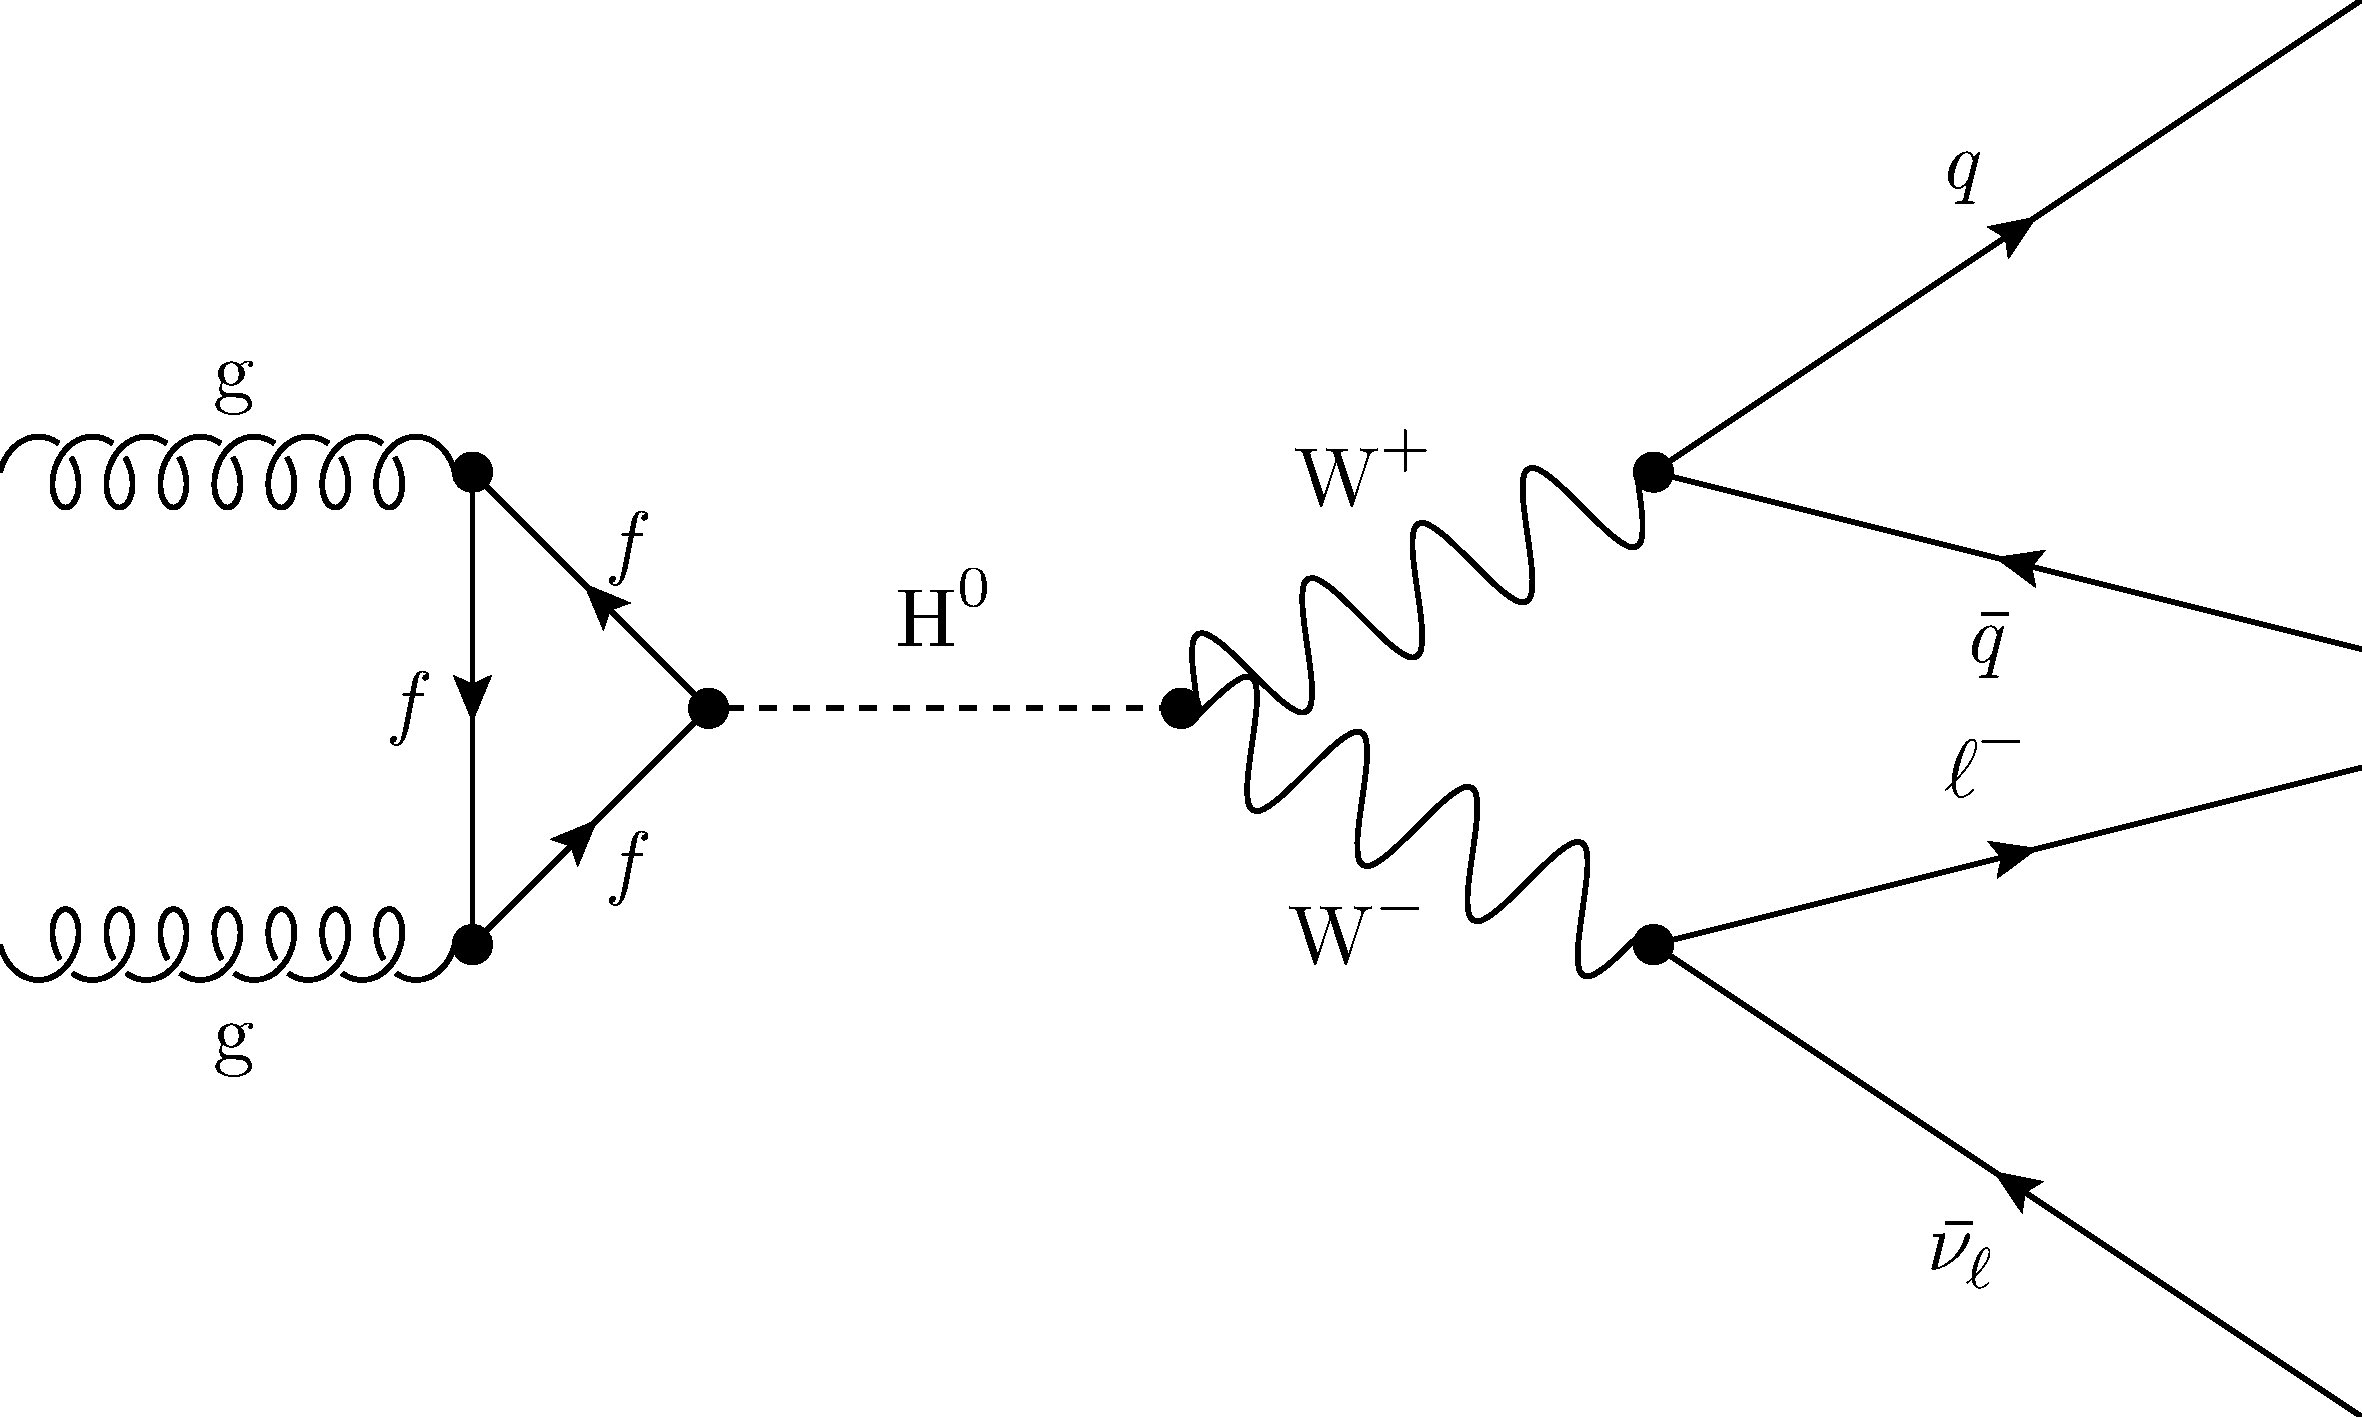
\includegraphics[width=\textwidth]{\figpath/FeynmanDiagrams/ggH_WW_lvjj.pdf}};}
				\only<5->{\node [inner sep=0pt,above right] {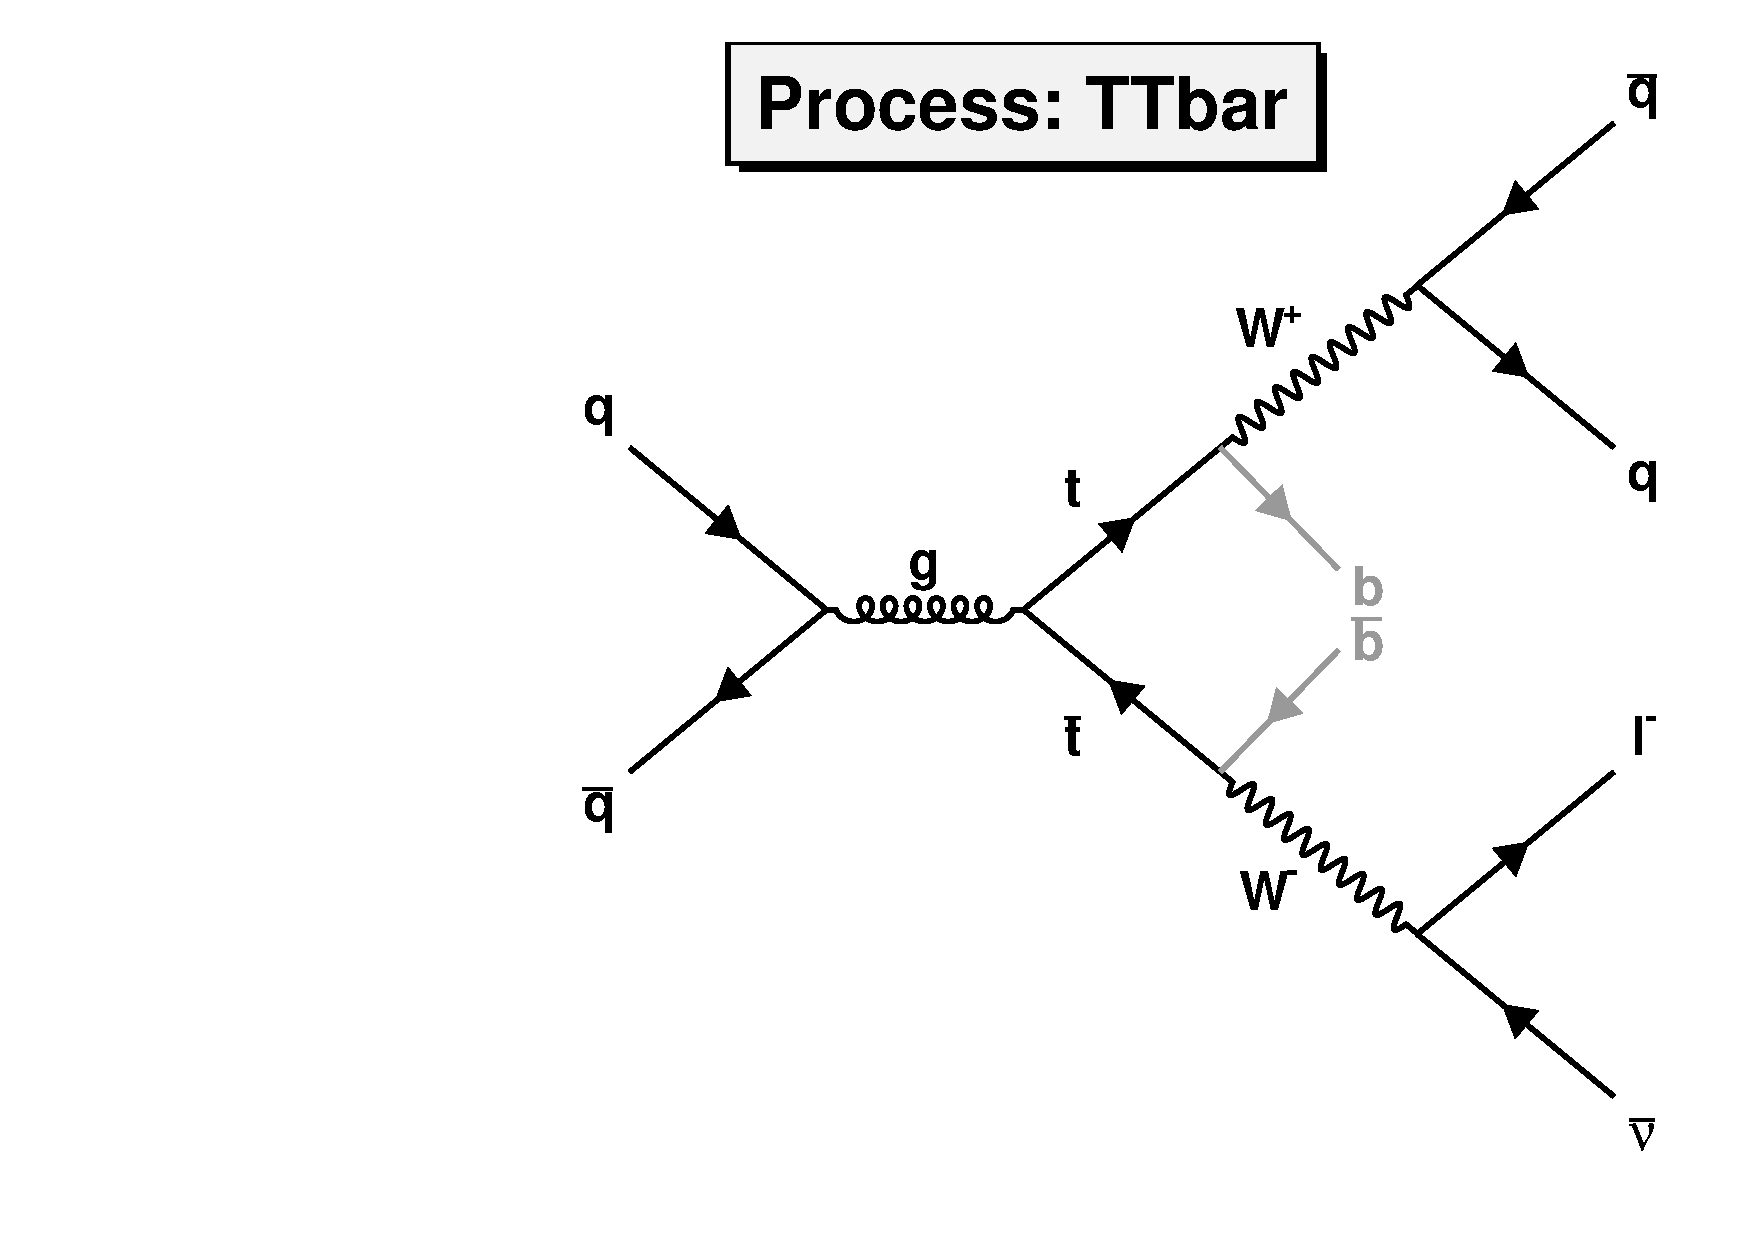
\includegraphics[width=\textwidth]{\figpath/FeynmanDiagrams/TTbar.pdf}};}
				%\only<6->{
				%	\node[rectangle, rounded corners, draw=red, very thick, anchor=base] (Irreducible) at (0,4) {%
				%		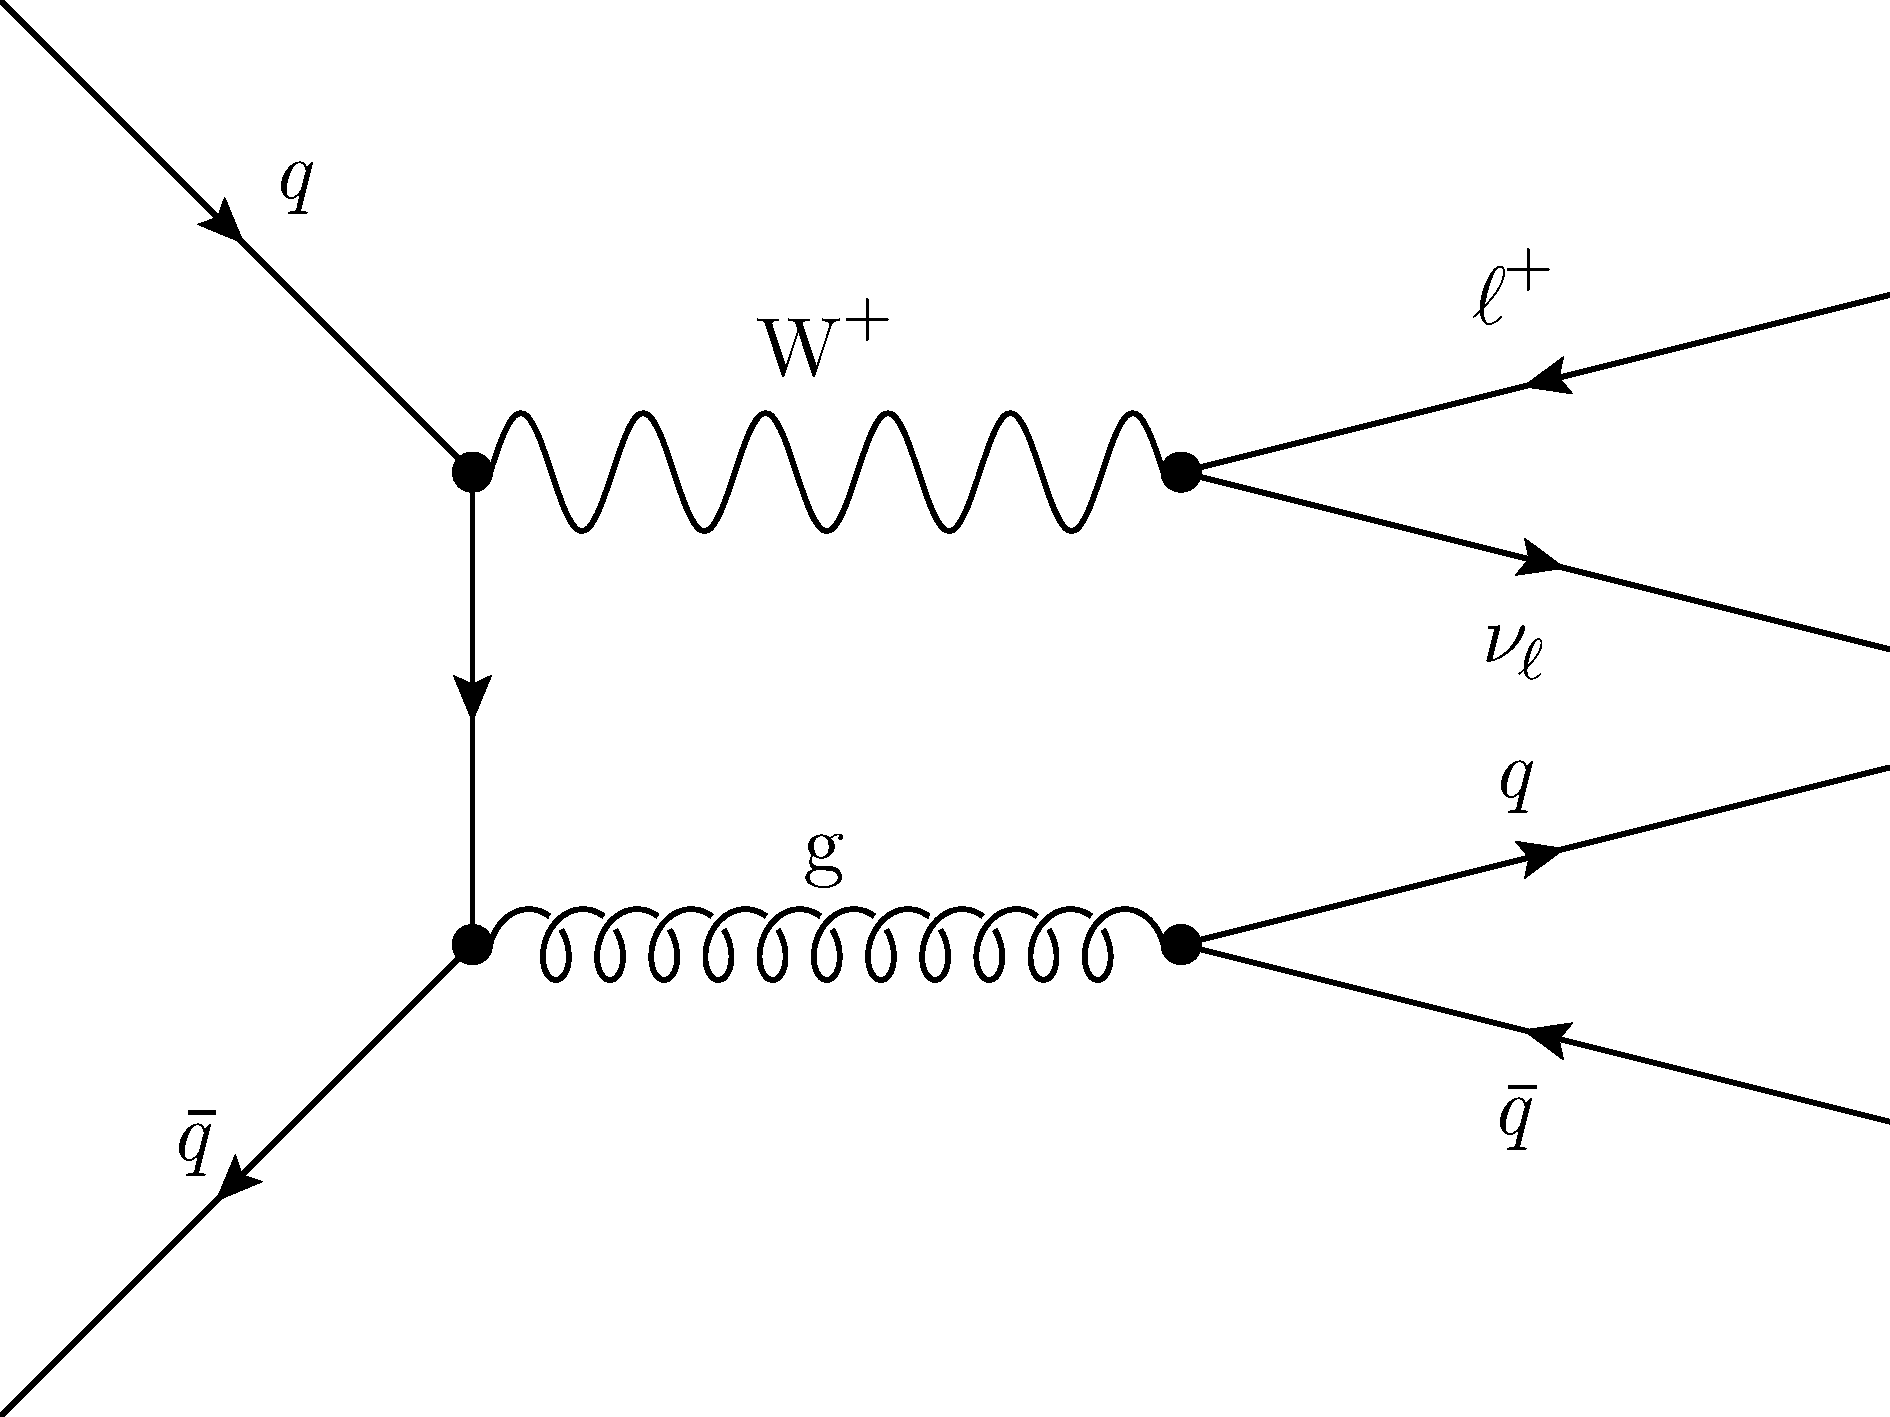
\includegraphics[width=0.48\textwidth]{\figpath/FeynmanDiagrams/WJets.pdf}
				%		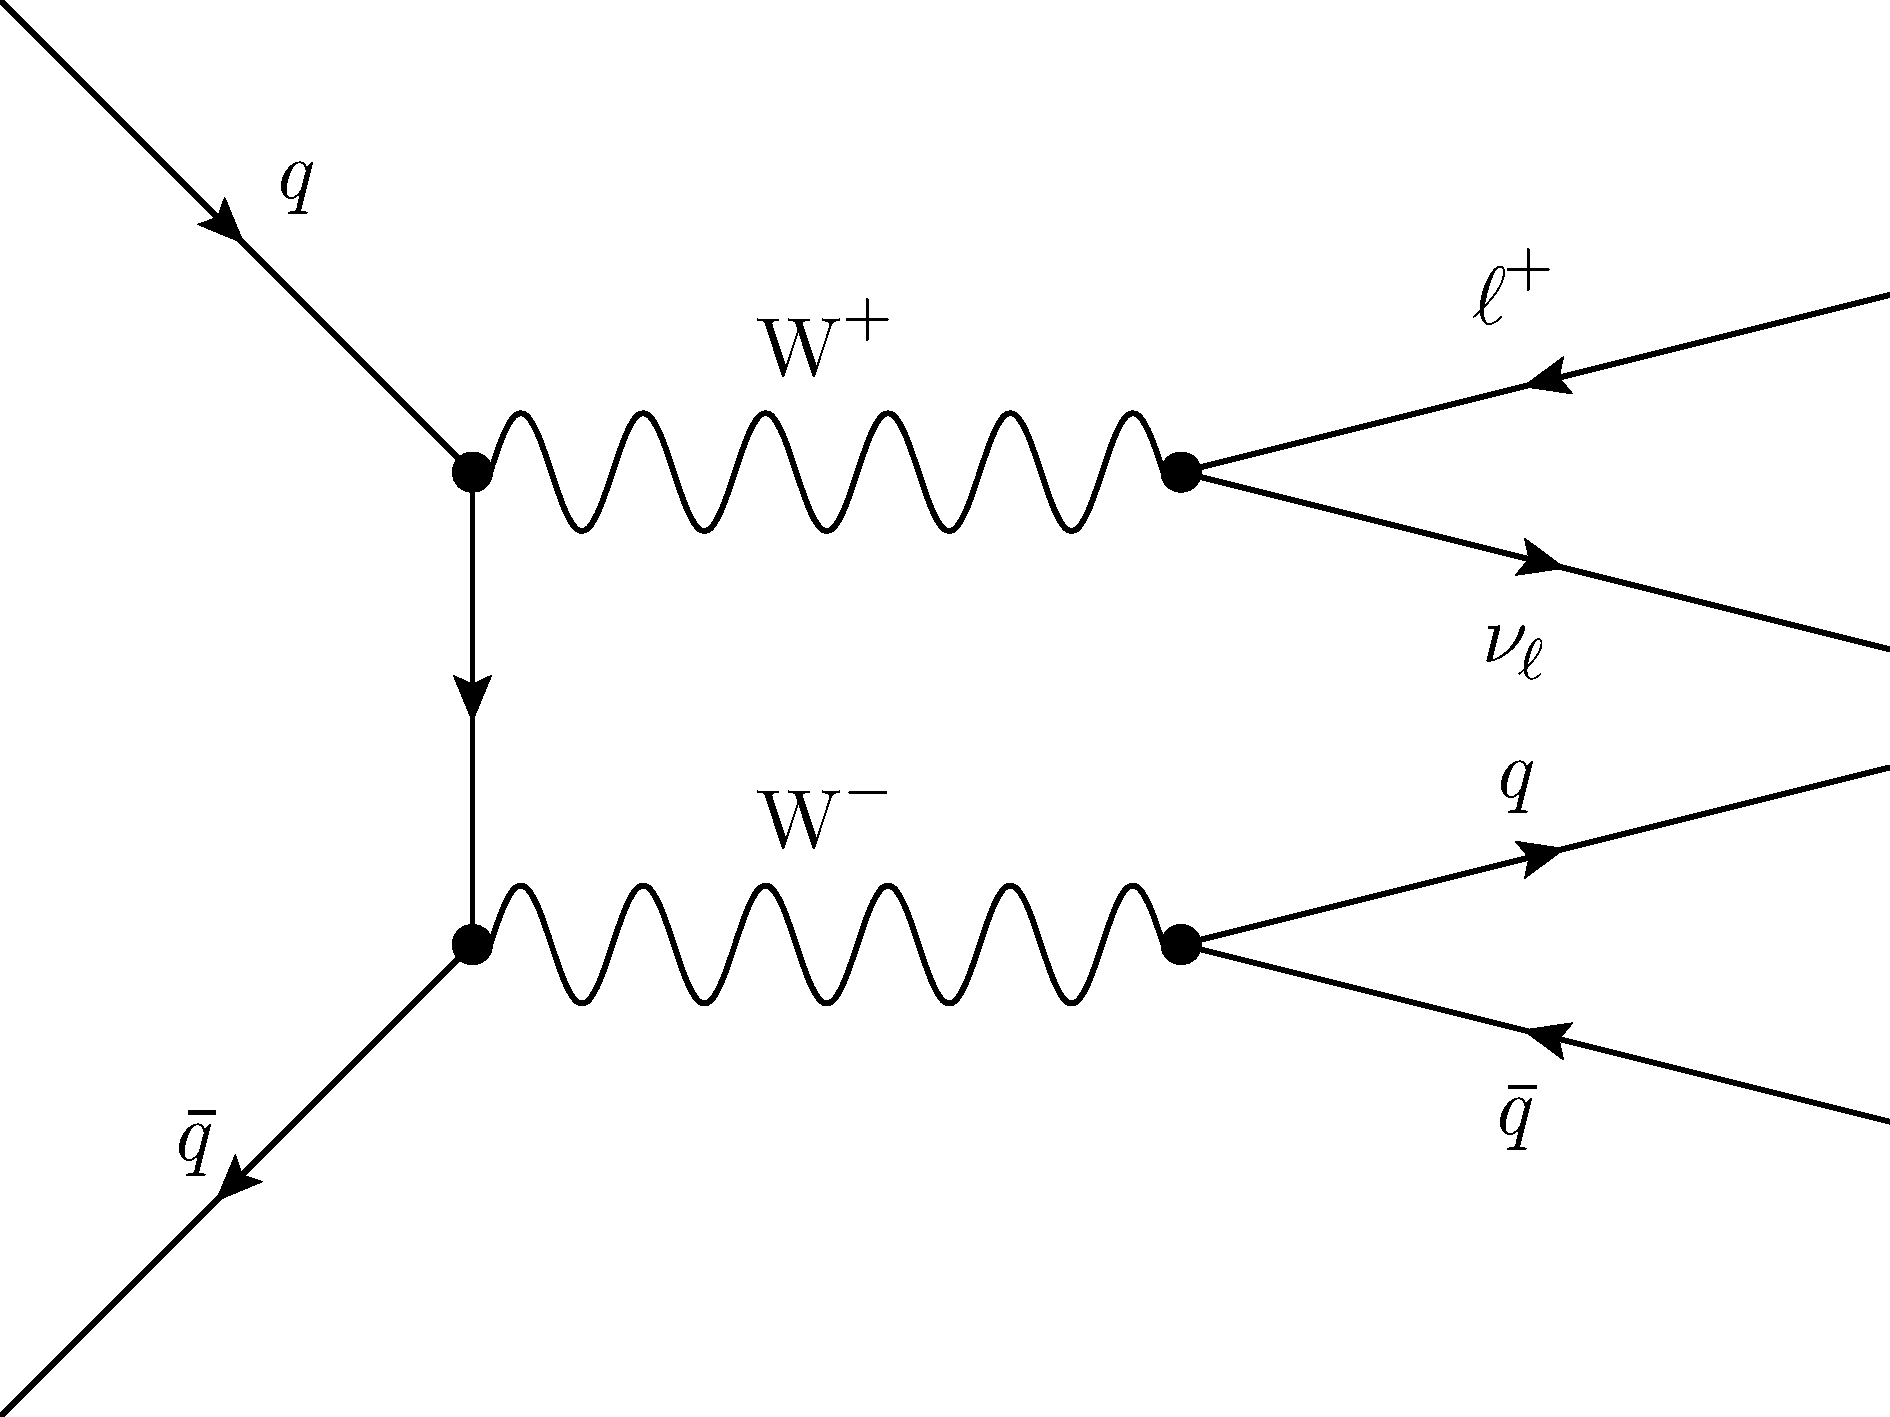
\includegraphics[width=0.48\textwidth]{\figpath/FeynmanDiagrams/WW.pdf}
				%	};
				%	\node[rectangle, rounded corners, draw=green, very thick, anchor=base] (Reducible1) at (0,2.4) {%
				%		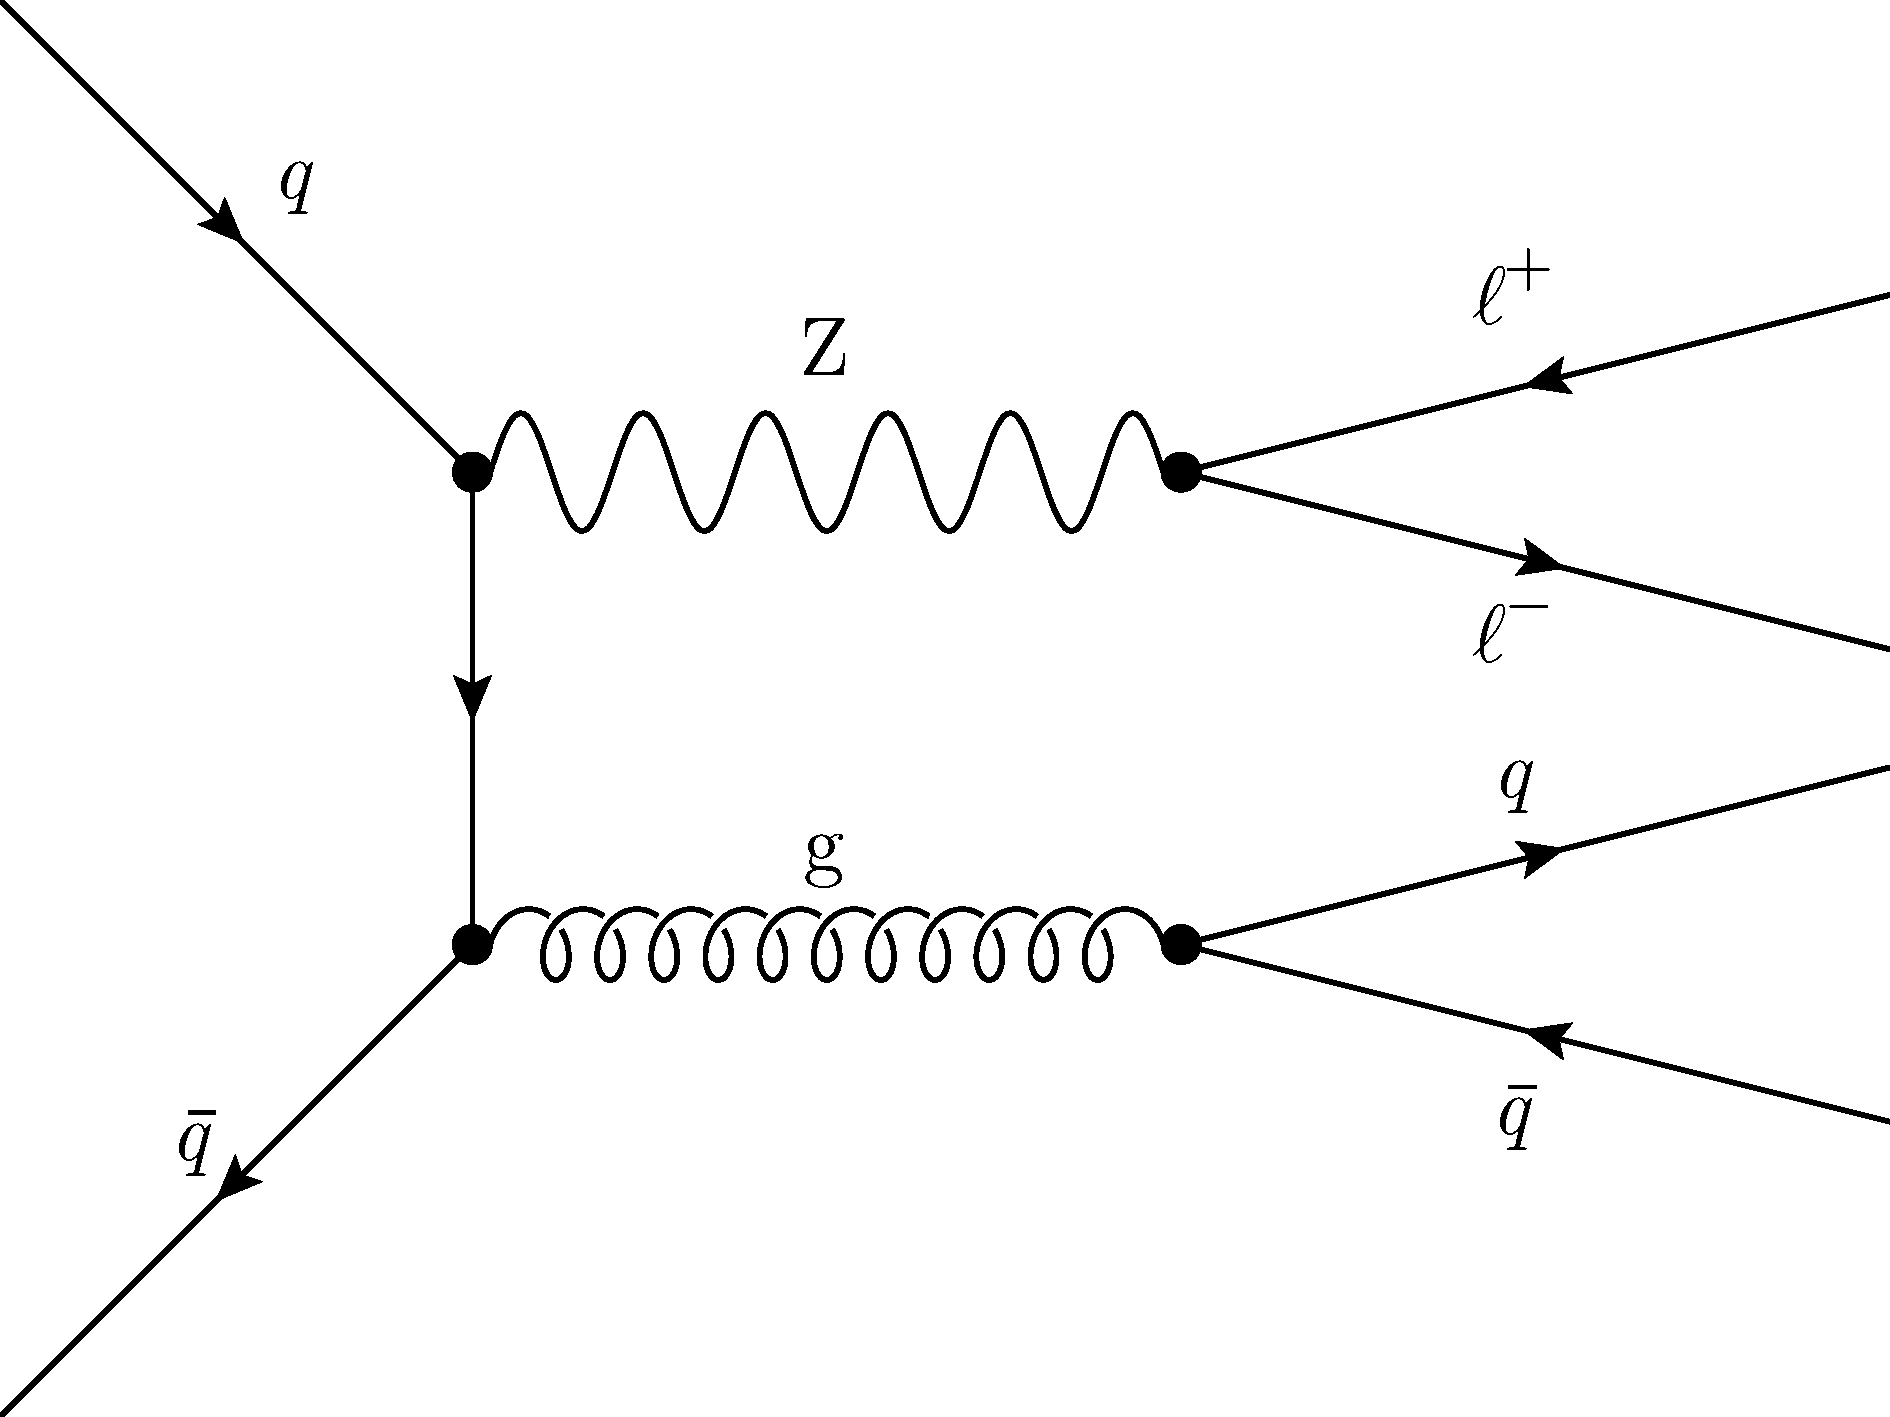
\includegraphics[width=0.31\textwidth]{\figpath/FeynmanDiagrams/ZJets.pdf}
				%		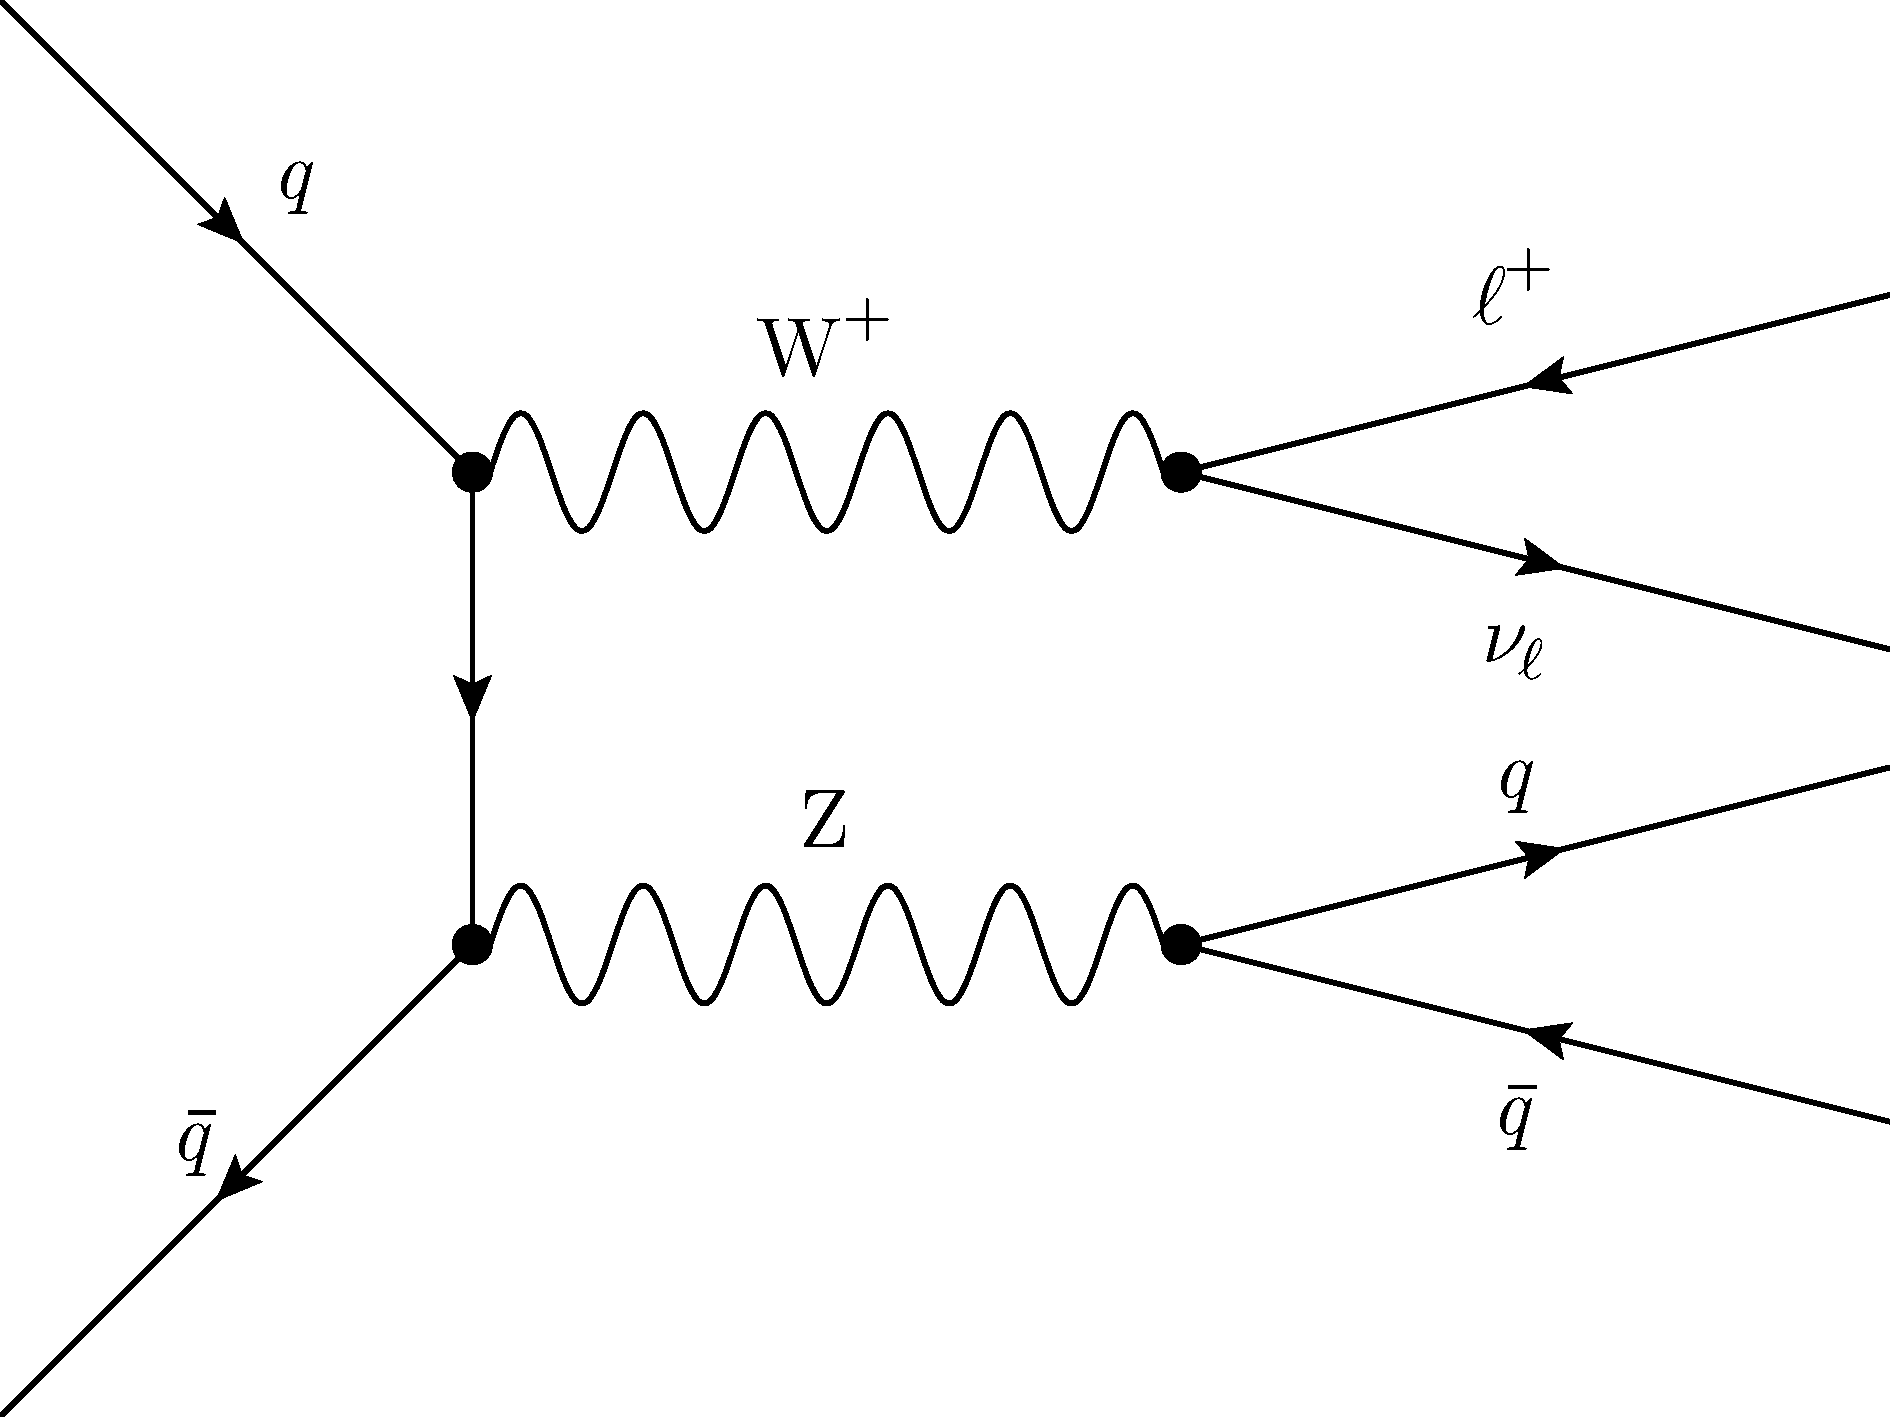
\includegraphics[width=0.31\textwidth]{\figpath/FeynmanDiagrams/WZ.pdf}
				%		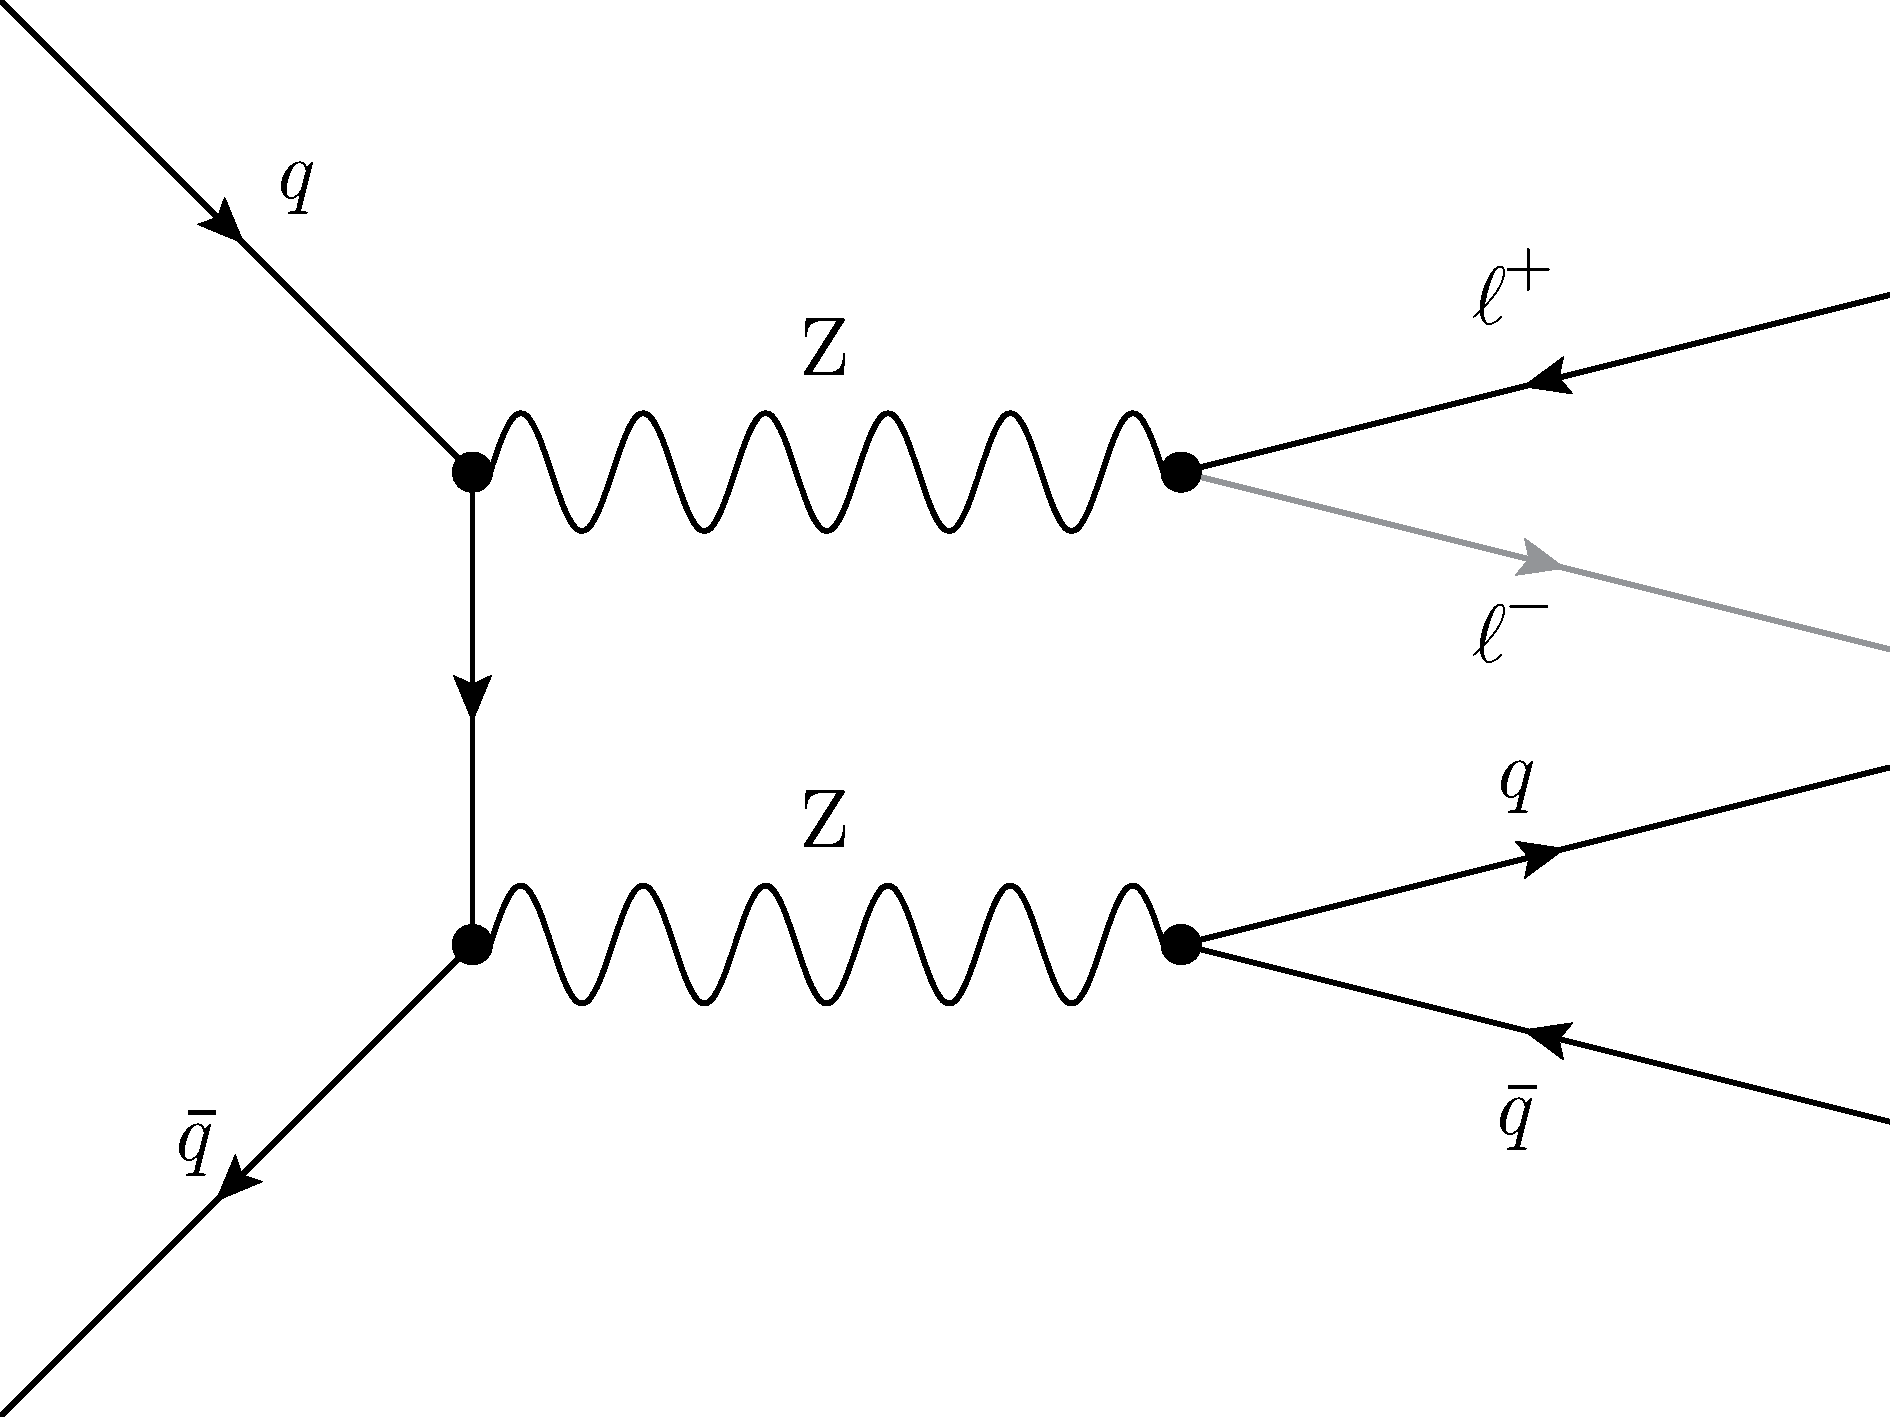
\includegraphics[width=0.31\textwidth]{\figpath/FeynmanDiagrams/ZZ.pdf}
				%	};
				%	\node[rectangle, rounded corners, draw=green, very thick, anchor=base] (Reducible2) at (0,0.5) {%
				%		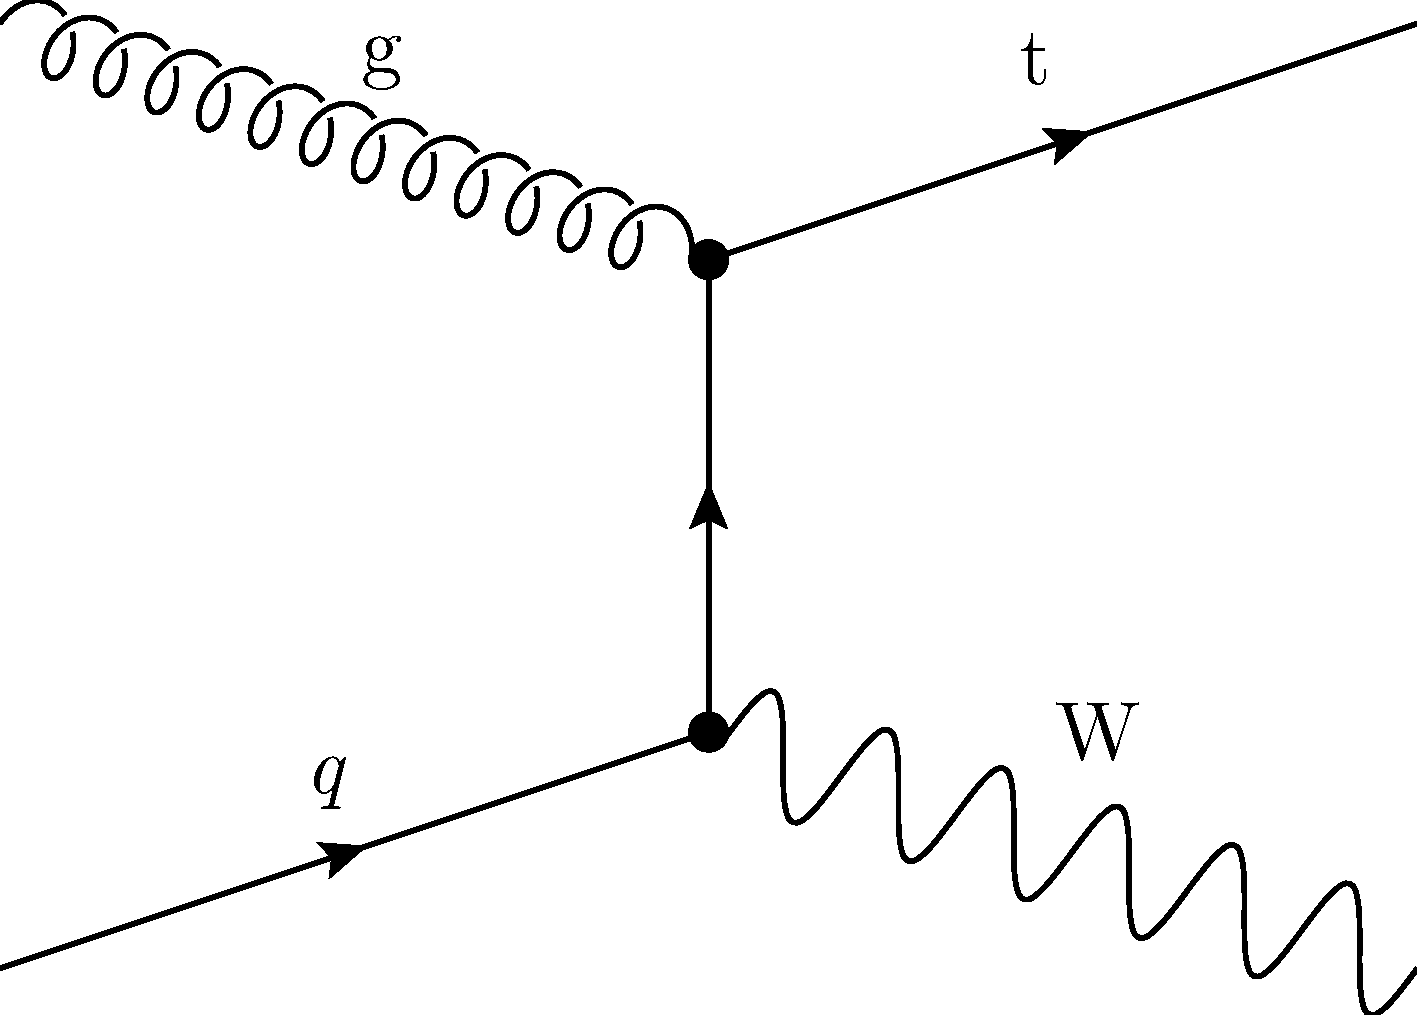
\includegraphics[width=0.31\textwidth]{\figpath/FeynmanDiagrams/STopTW.pdf}
				%		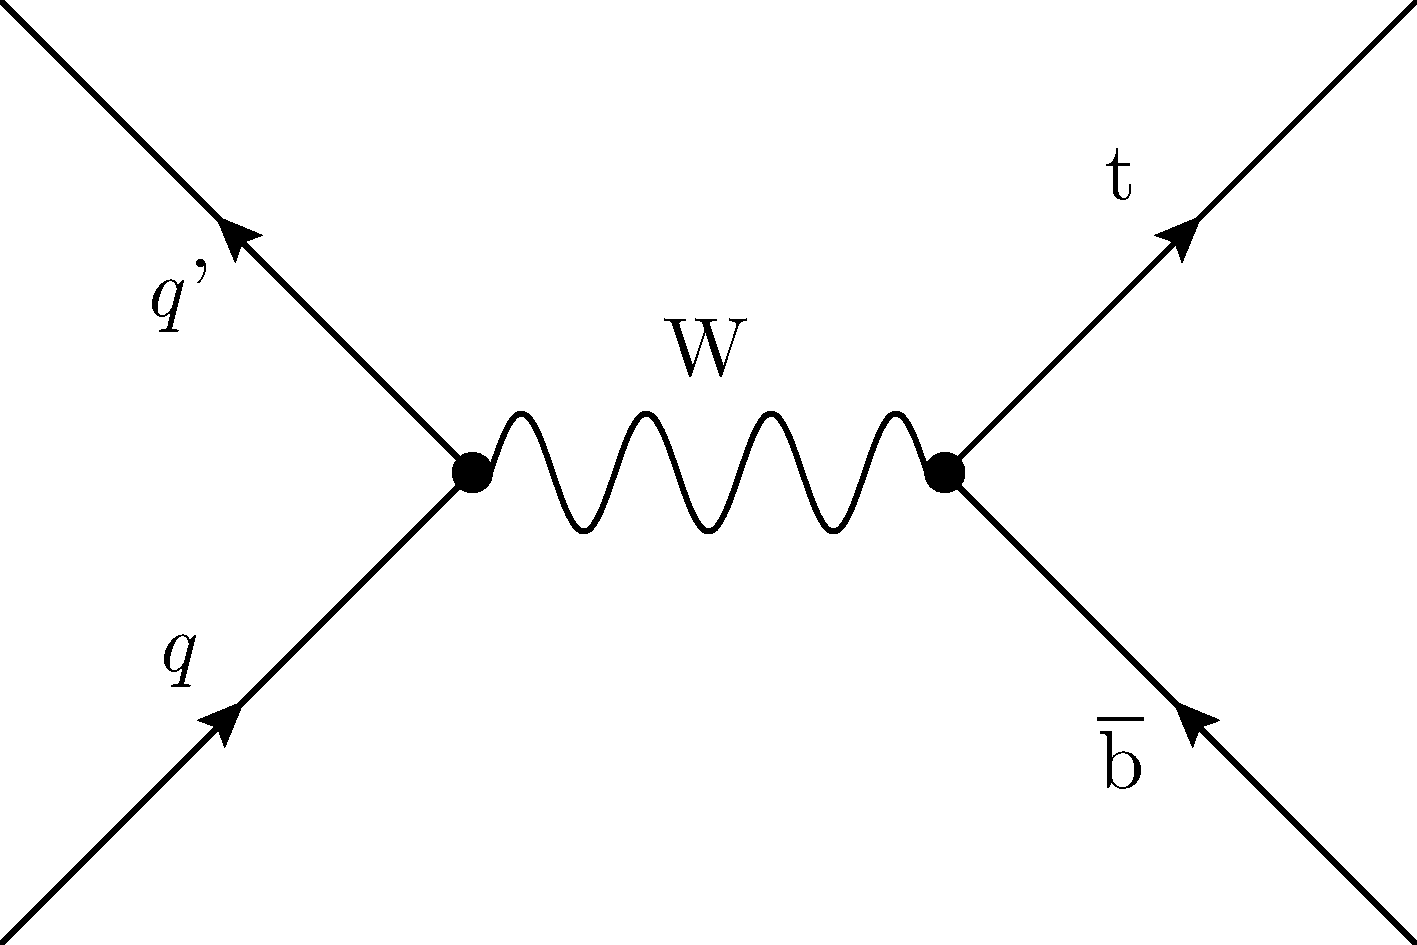
\includegraphics[width=0.31\textwidth]{\figpath/FeynmanDiagrams/STopS.pdf}
				%		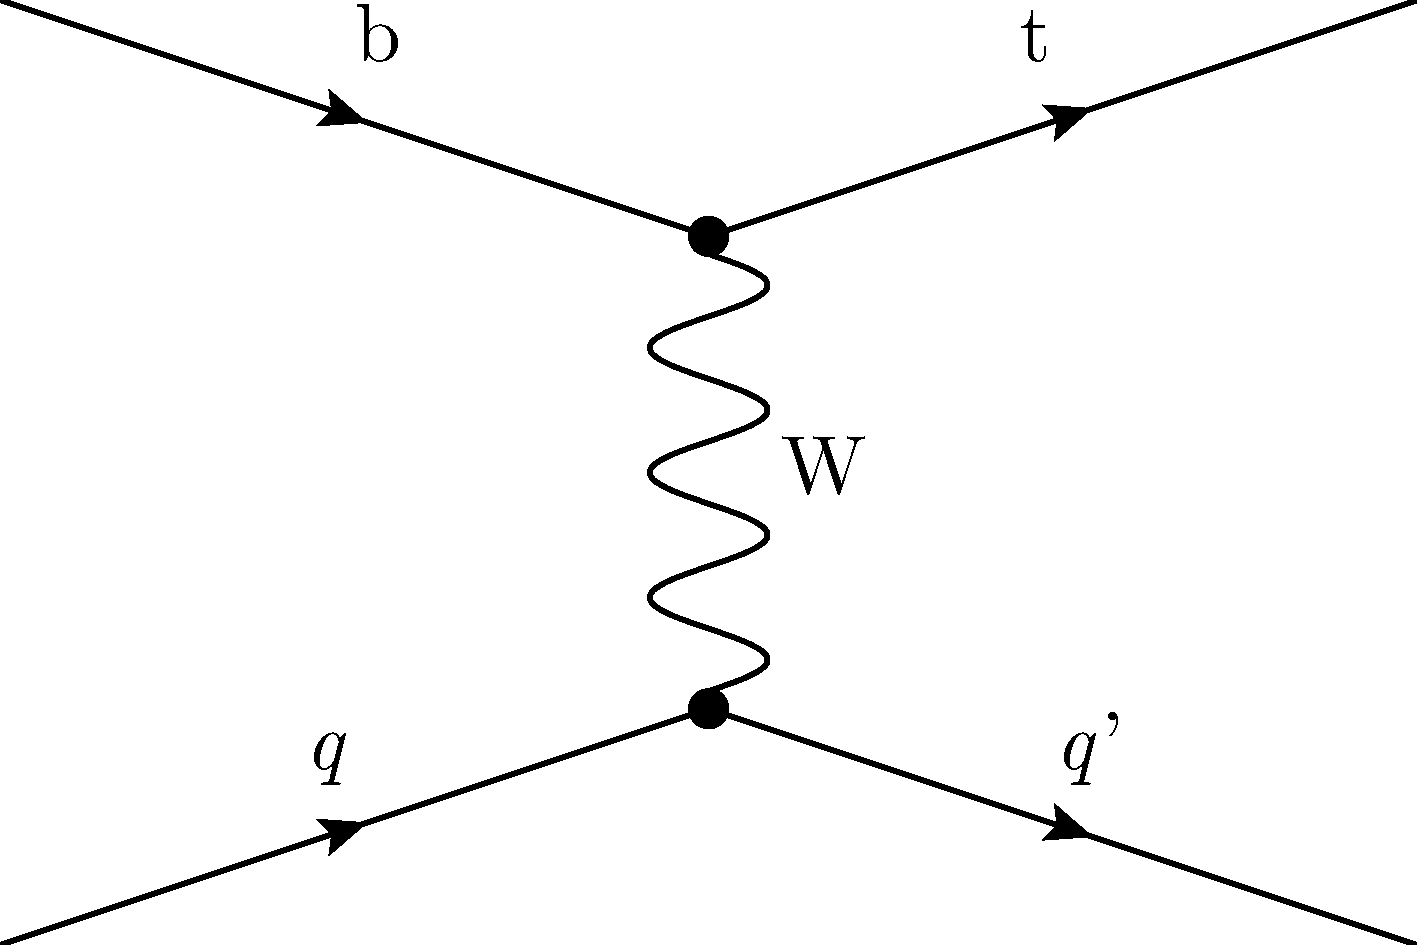
\includegraphics[width=0.31\textwidth]{\figpath/FeynmanDiagrams/STopT.pdf}
				%	};
				%	\node[rectangle, rounded corners, draw=green, very thick, anchor=base] (Reducible3) at (0,-1.5) {%
				%		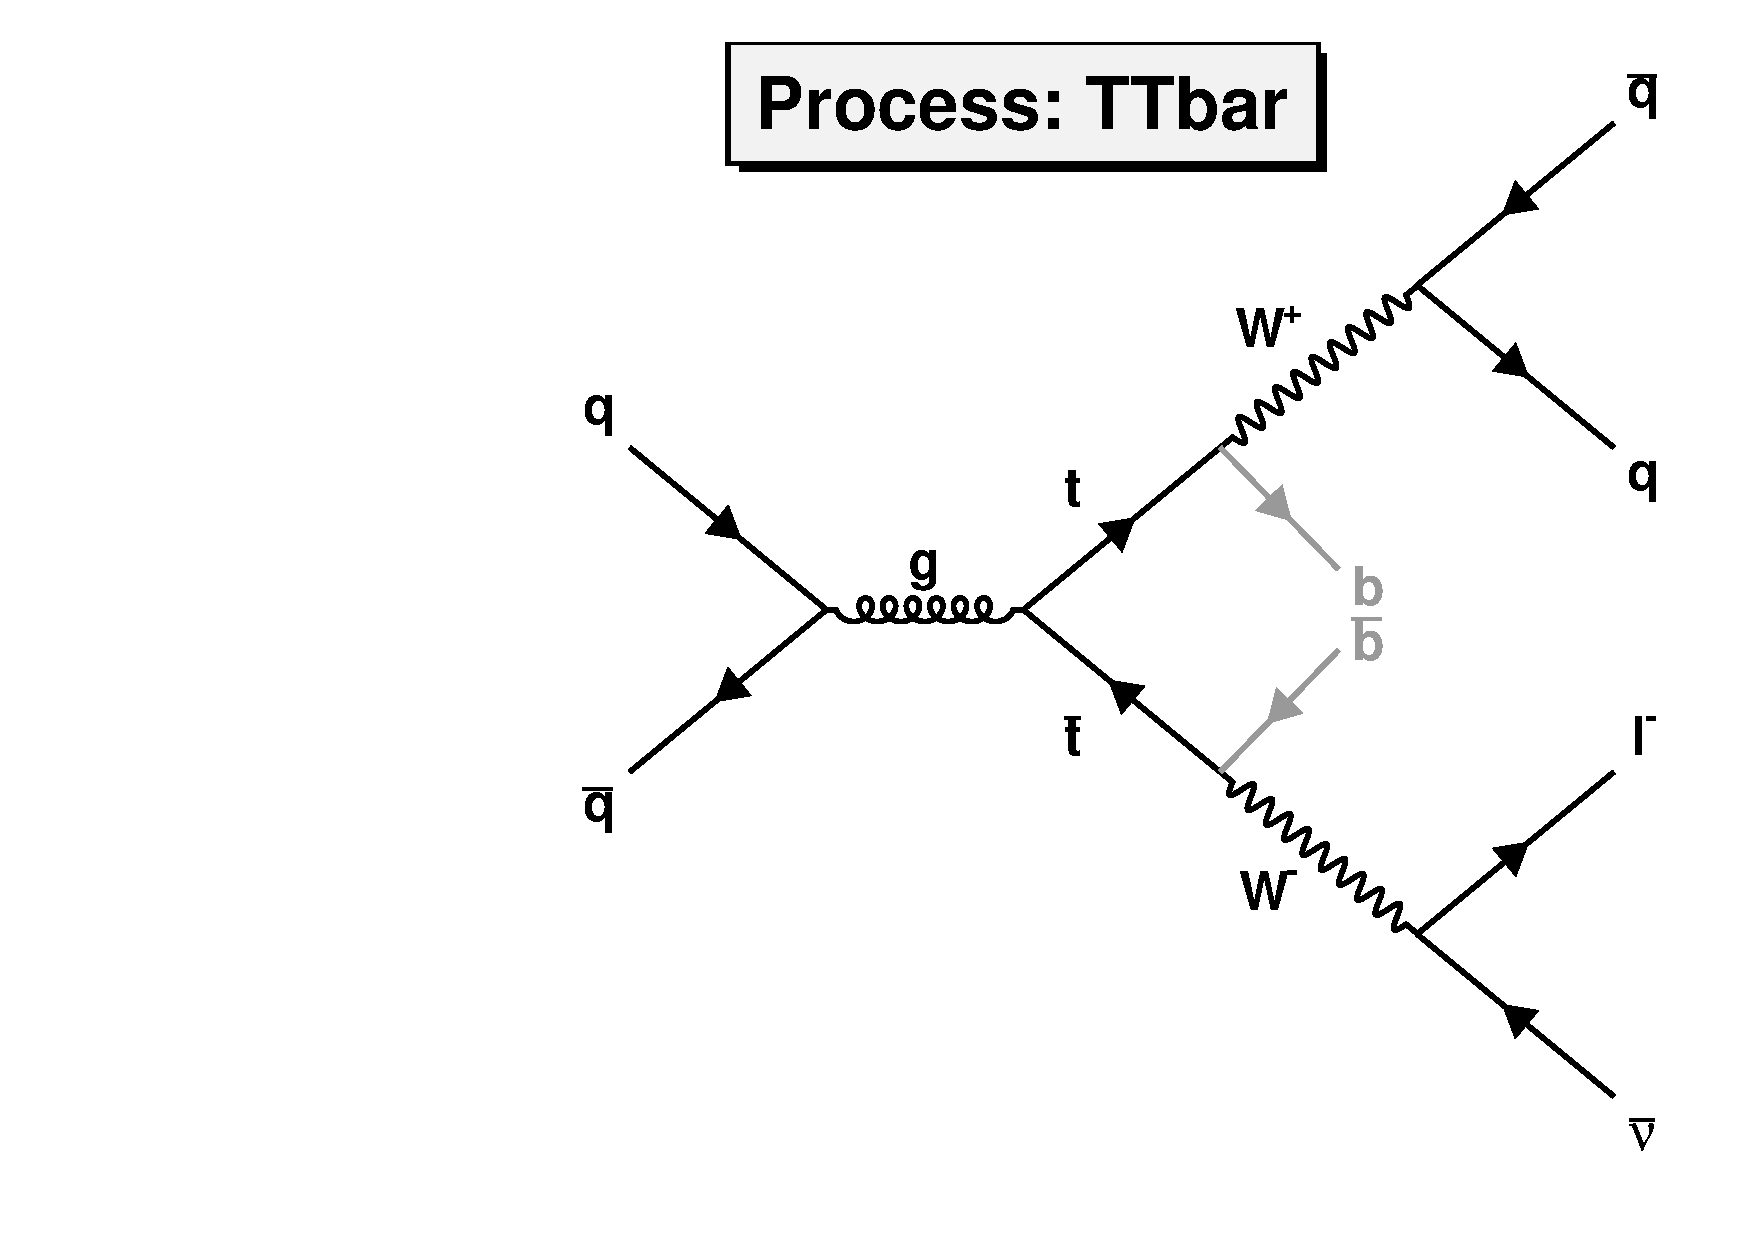
\includegraphics[width=0.31\textwidth]{\figpath/FeynmanDiagrams/TTbar.pdf}
				%		%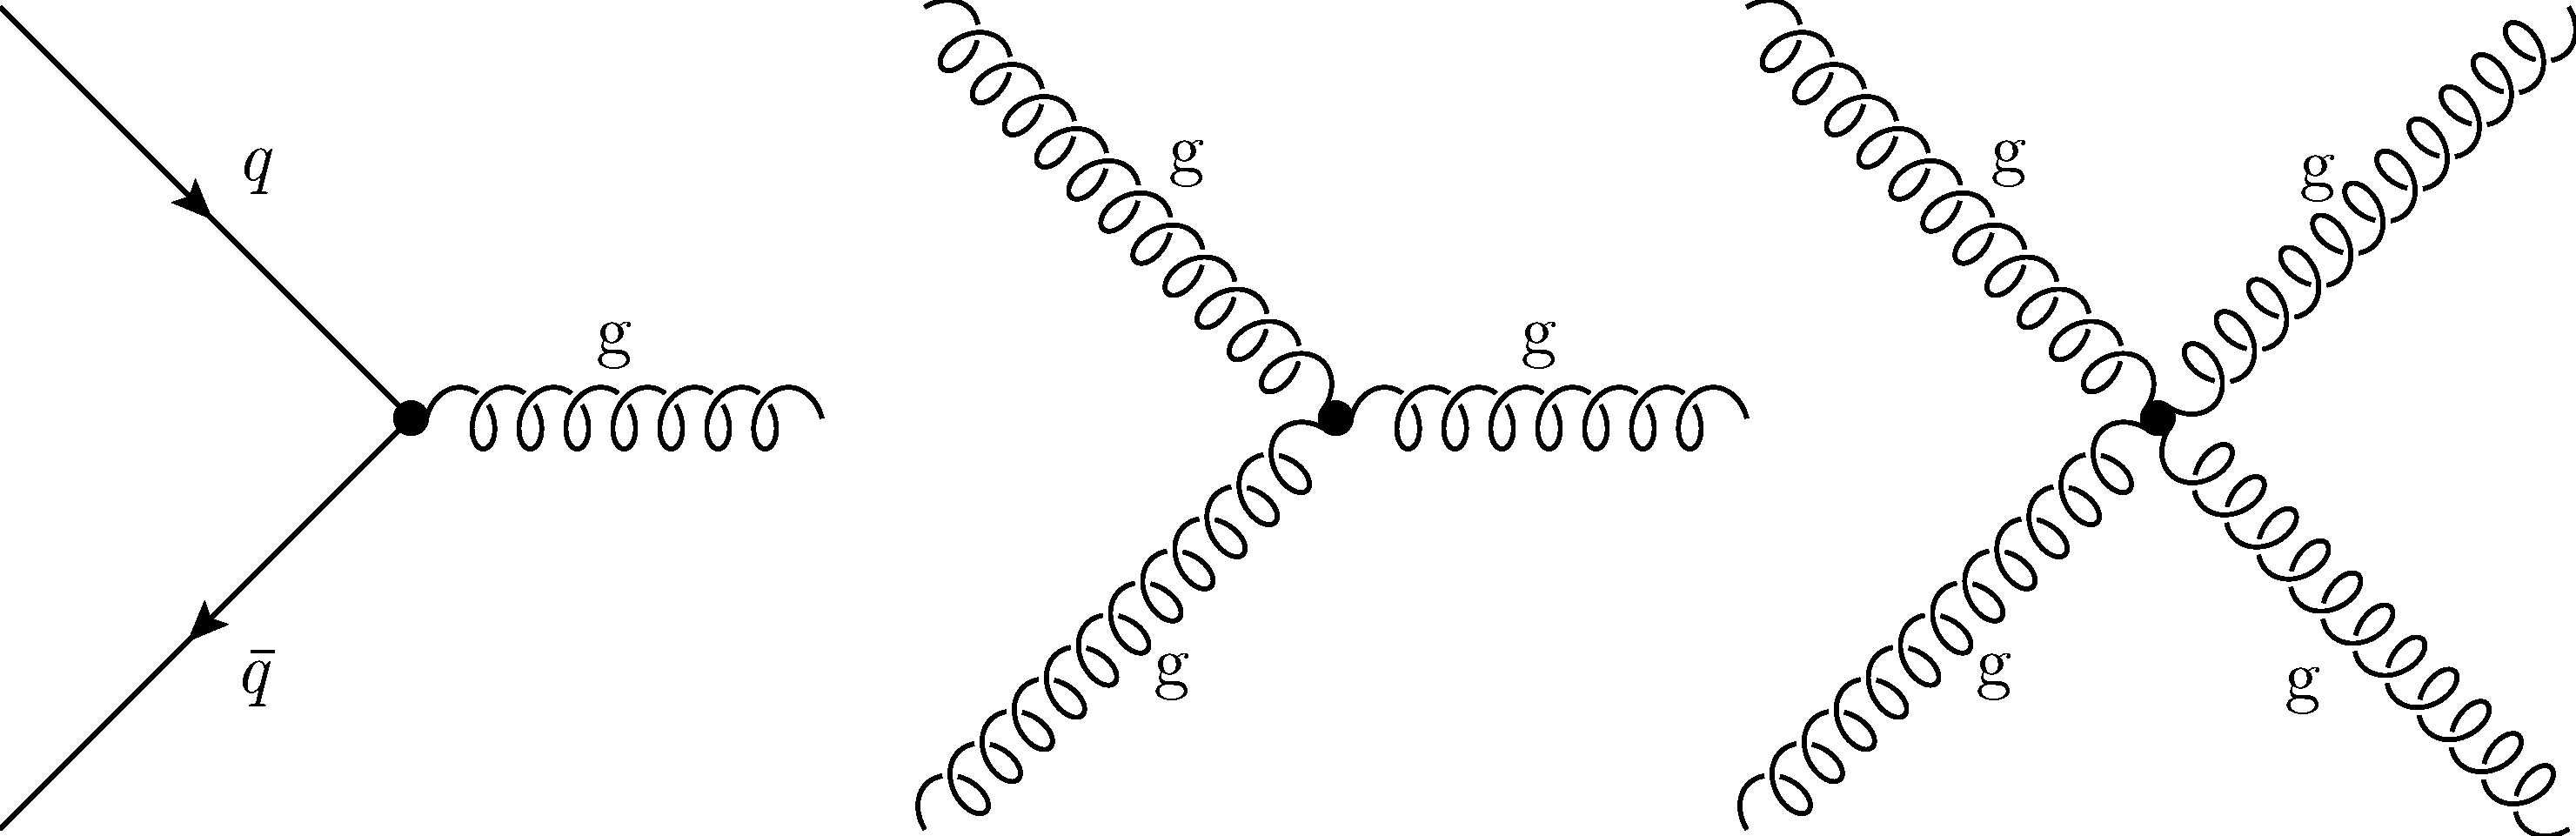
\includegraphics[width=0.48\textwidth]{\figpath/FeynmanDiagrams/QCD.pdf}
				%	};
				%}
				% define destination coordinates
				\only<2>{\node[rectangle, rounded corners, draw=red, very thick, minimum height=1em, text width=1.15em, anchor=base] (lepton) at (4.6,1.5) {};}
				\only<3>{
					\node[rectangle, rounded corners, draw=blue, very thick, minimum height=1em, text width=1.15em, anchor=base] (jet1) at (4.6,2.9) {};
					\node[rectangle, rounded corners, draw=blue, very thick, minimum height=1em, text width=1.15em, anchor=base] (jet2) at (4.6,1.8) {};
				}
				\only<4>{\node[rectangle, rounded corners, draw=ForestGreen, very thick, minimum height=1em, text width=1.15em, anchor=base] (met) at (4.6,0.4) {};}
				\only<5>{\node[rectangle, rounded corners, draw=violet, very thick, minimum height=2em, text width=1em, anchor=base] (bjet) at (3.35,2.3) {};}
			\end{tikzpicture}
		\end{column}
	\end{columns}
	% define overlays
	% Note the use of the overlay option. This is required when 
	% you want to access nodes in different pictures.
	\only<2-5>{
	\begin{tikzpicture}[overlay]
			\only<2>{\path[->,red,thick] ([xshift=1mm,yshift=1mm]s-lepton) edge [out=0,in=180] (lepton);}
			\only<3>{
				\path[->,blue,thick] ([xshift=1mm,yshift=1mm]s-jet) edge [out=0,in=180] (jet1);
				\path[->,blue,thick] ([xshift=1mm,yshift=1mm]s-jet) edge [out=0,in=180] (jet2);
			}
			\only<4>{\path[->,ForestGreen,thick] ([xshift=1mm,yshift=1mm]s-met) edge [out=0,in=180] (met);}
			\only<5>{\path[->,violet,thick] ([xshift=1mm,yshift=1mm]s-bjet) edge [out=0,in=180] (bjet);}
	\end{tikzpicture}
	}
\end{frame}
%\againframe<2>{frame:event_signature}
%\againframe<3>{frame:event_signature}
%\againframe<4>{frame:event_signature}
%\againframe<5>{frame:event_signature}
%\againframe<6>{frame:event_signature}


%%--------------------------------------------------------------------------------------------

\subsection*{SM Backgrounds}

%%--------------------------------------------------------------------------------------------

\begin{frame}
	\frametitle{SM Backgrounds}
	\vspace*{-0.24cm}
	\begin{itemize}
		\item \textit{\textbf{Irreducible}} backgrounds are those with real leptons and no b-jets
	\end{itemize}
	\vspace*{-0.2cm}
	\begin{table}[tb]
		\centering
		\begin{tabular}{>{\centering}m{0.15\textwidth} >{\centering}m{0.27\textwidth} | >{\centering}m{0.15\textwidth} >{\centering\arraybackslash}m{0.27\textwidth}}
			\Wjets & 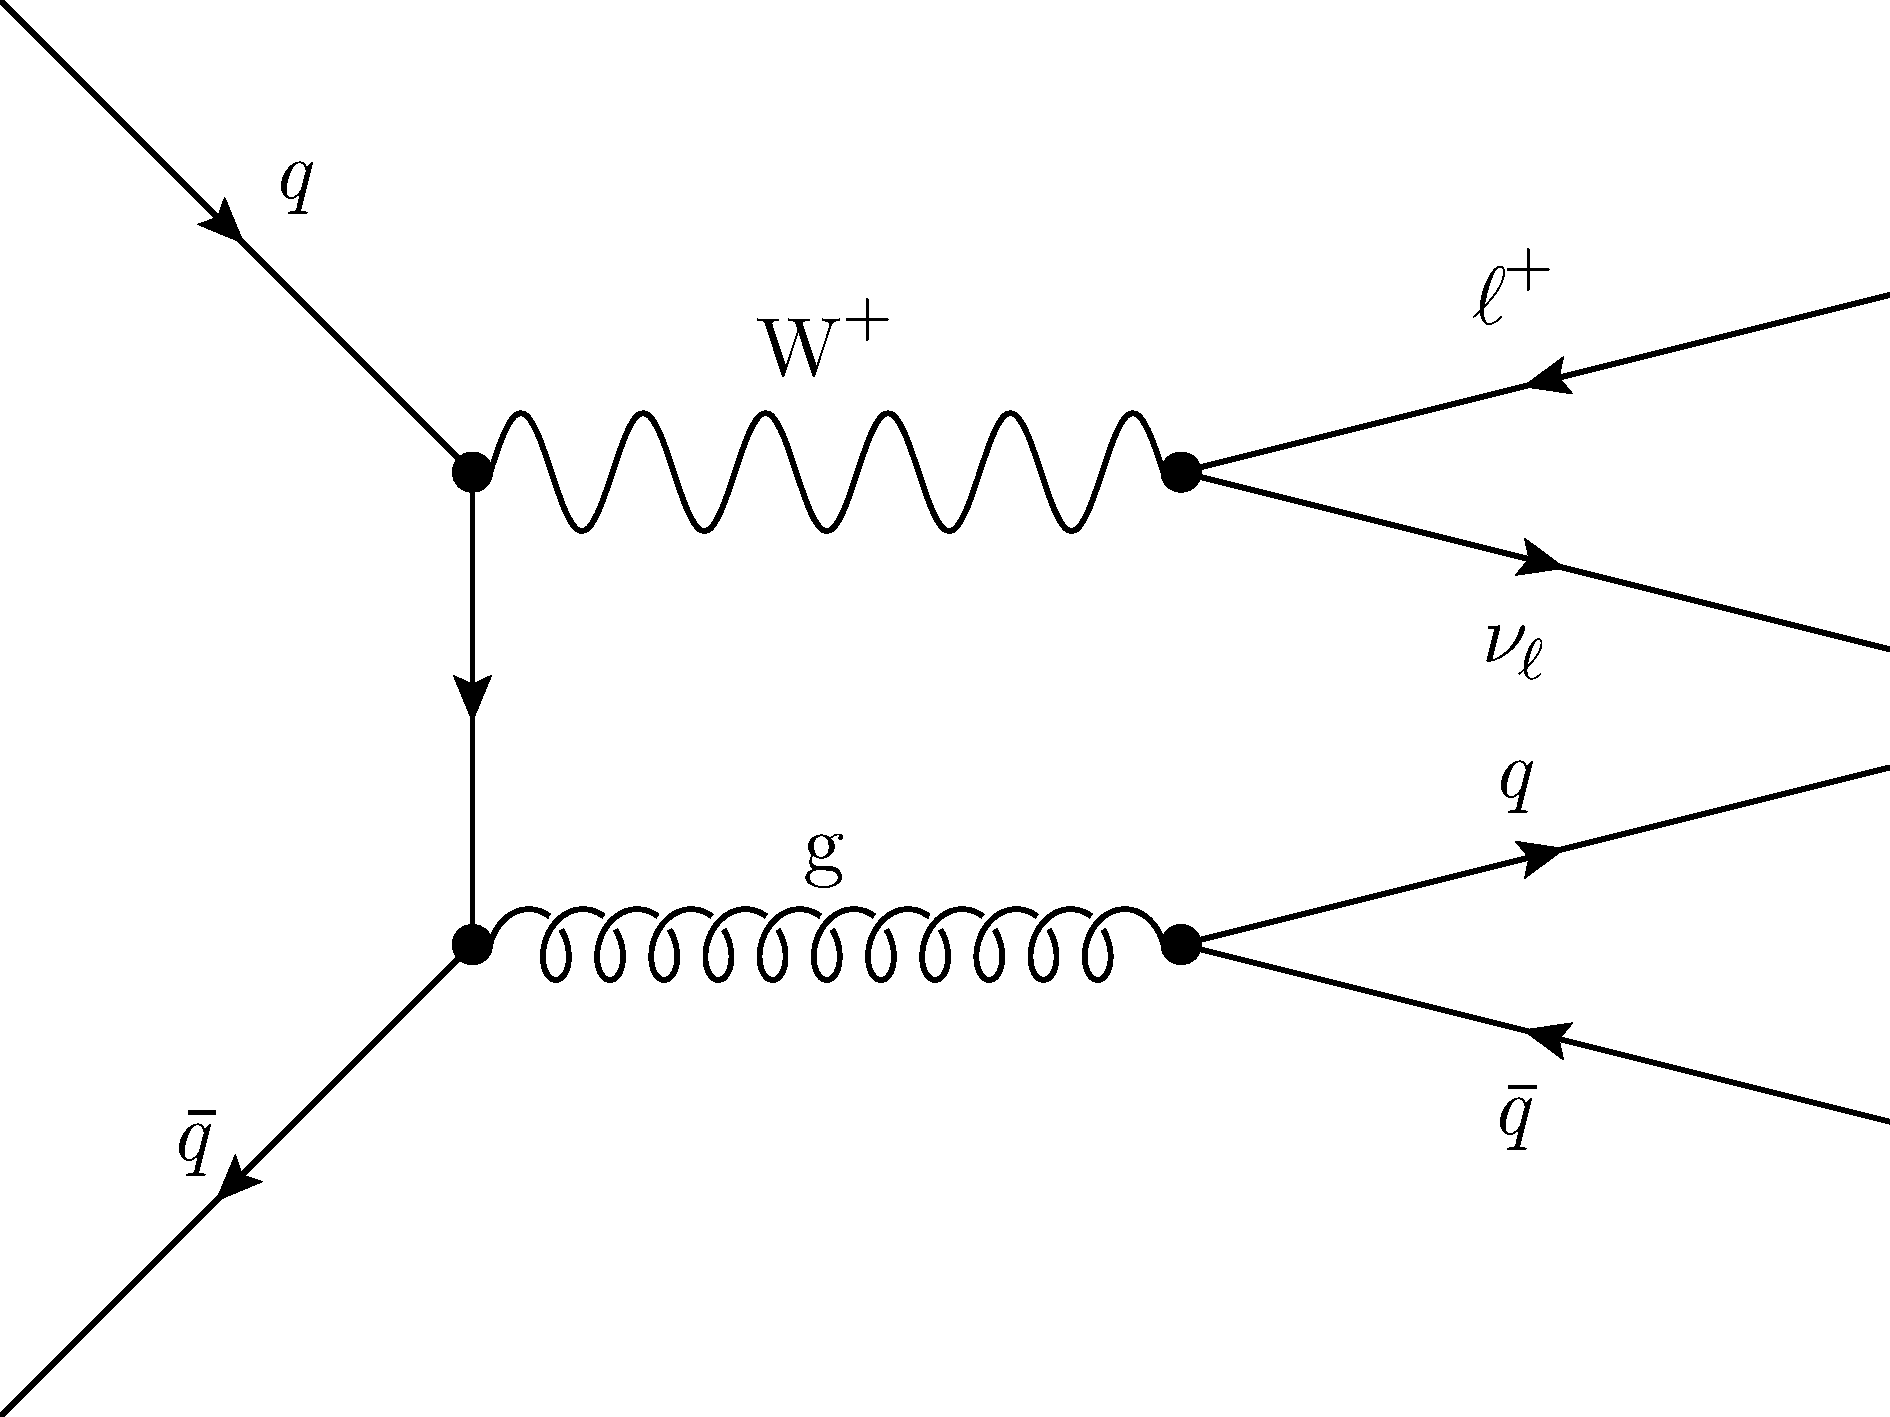
\includegraphics[width=0.25\textwidth]{\figpath/FeynmanDiagrams/WJets.pdf} & \WW & 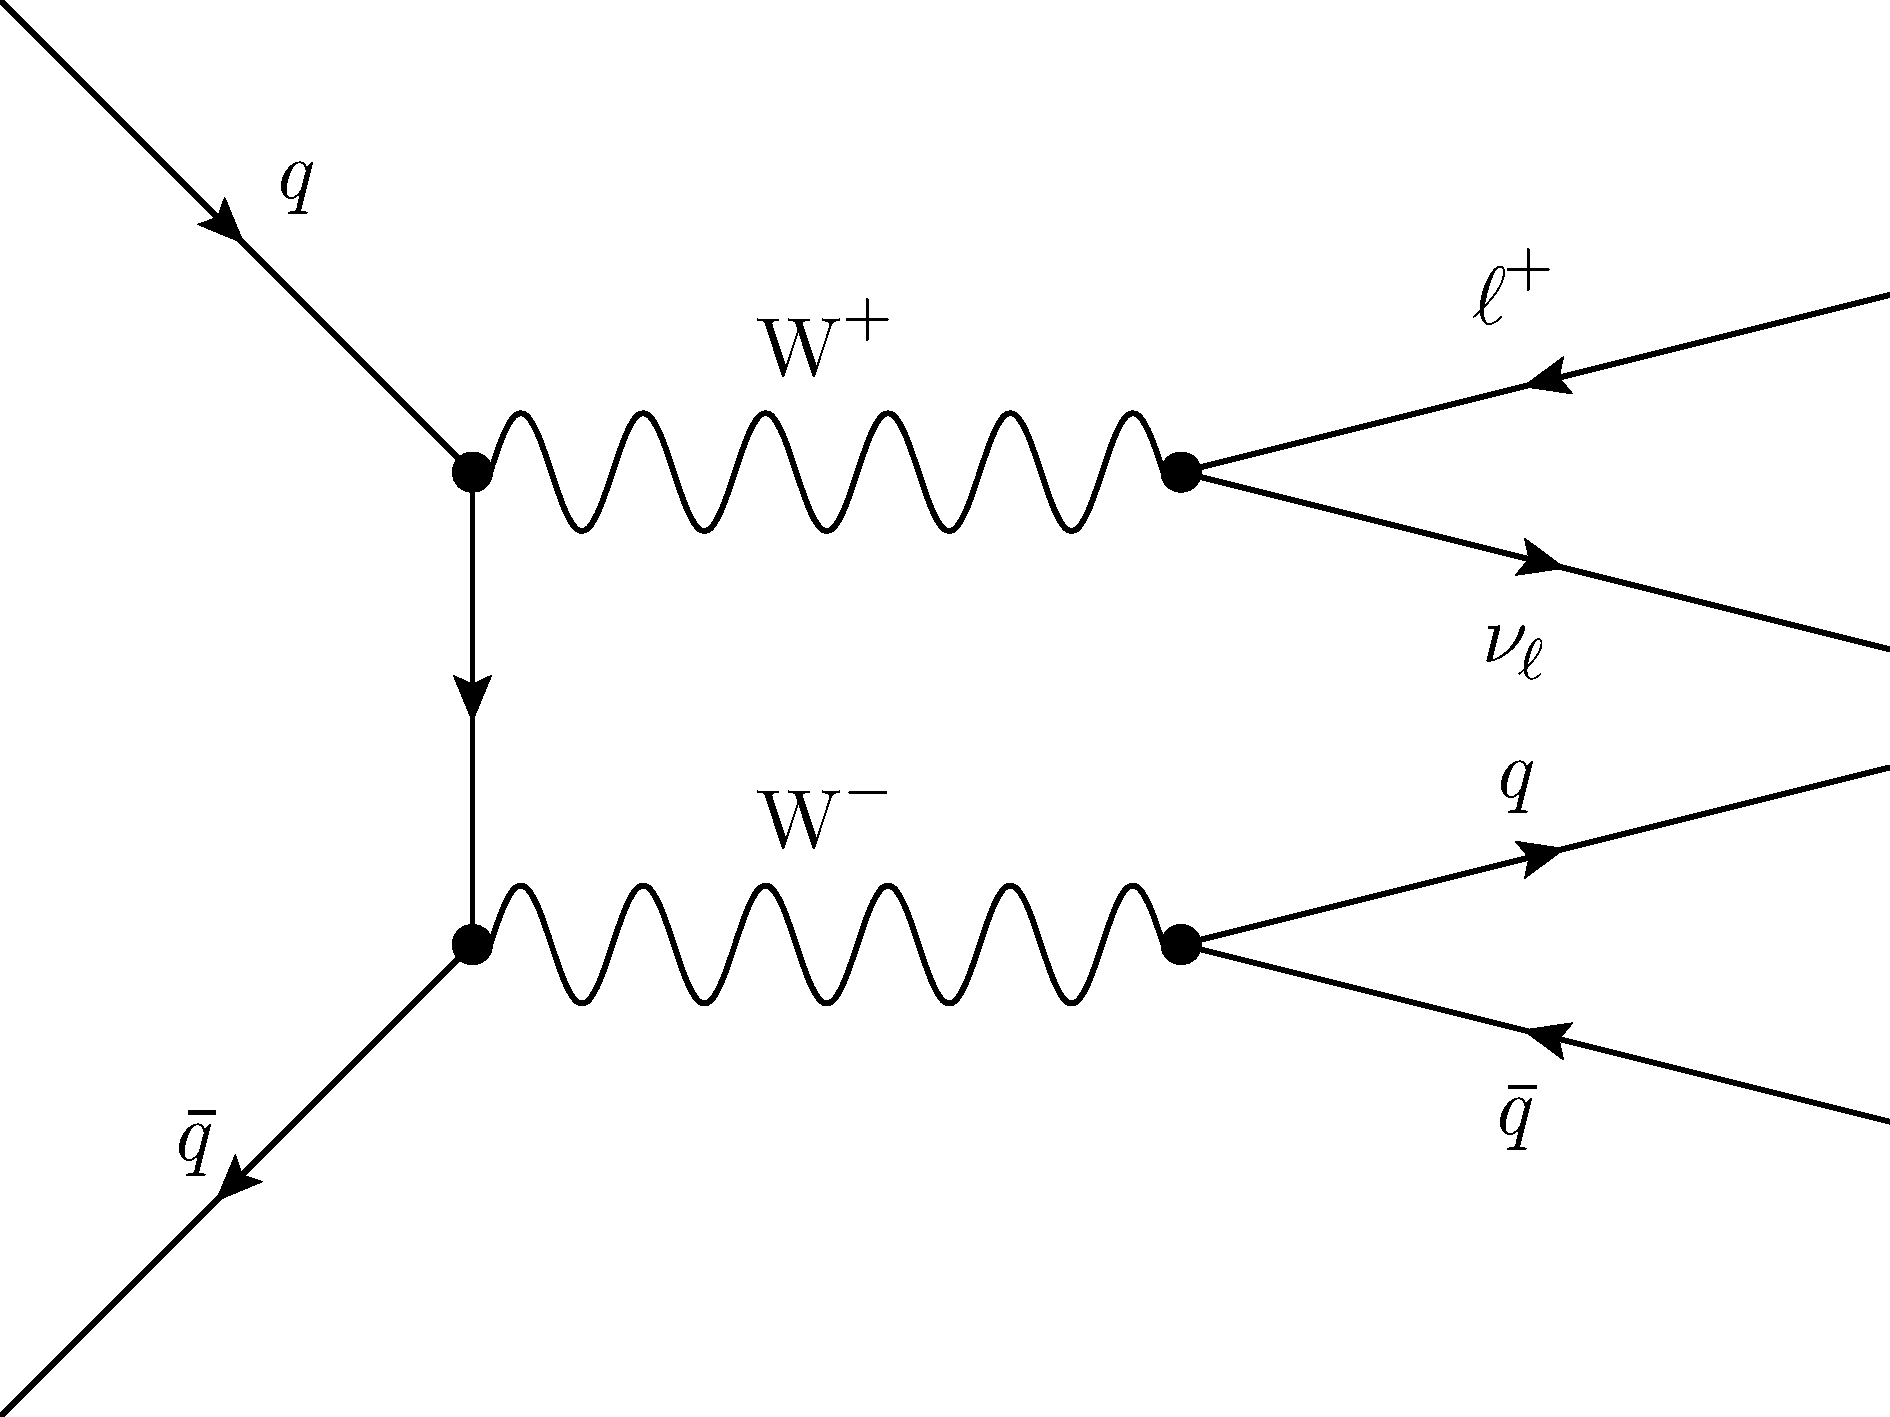
\includegraphics[width=0.25\textwidth]{\figpath/FeynmanDiagrams/WW.pdf} \\
			\WZ & 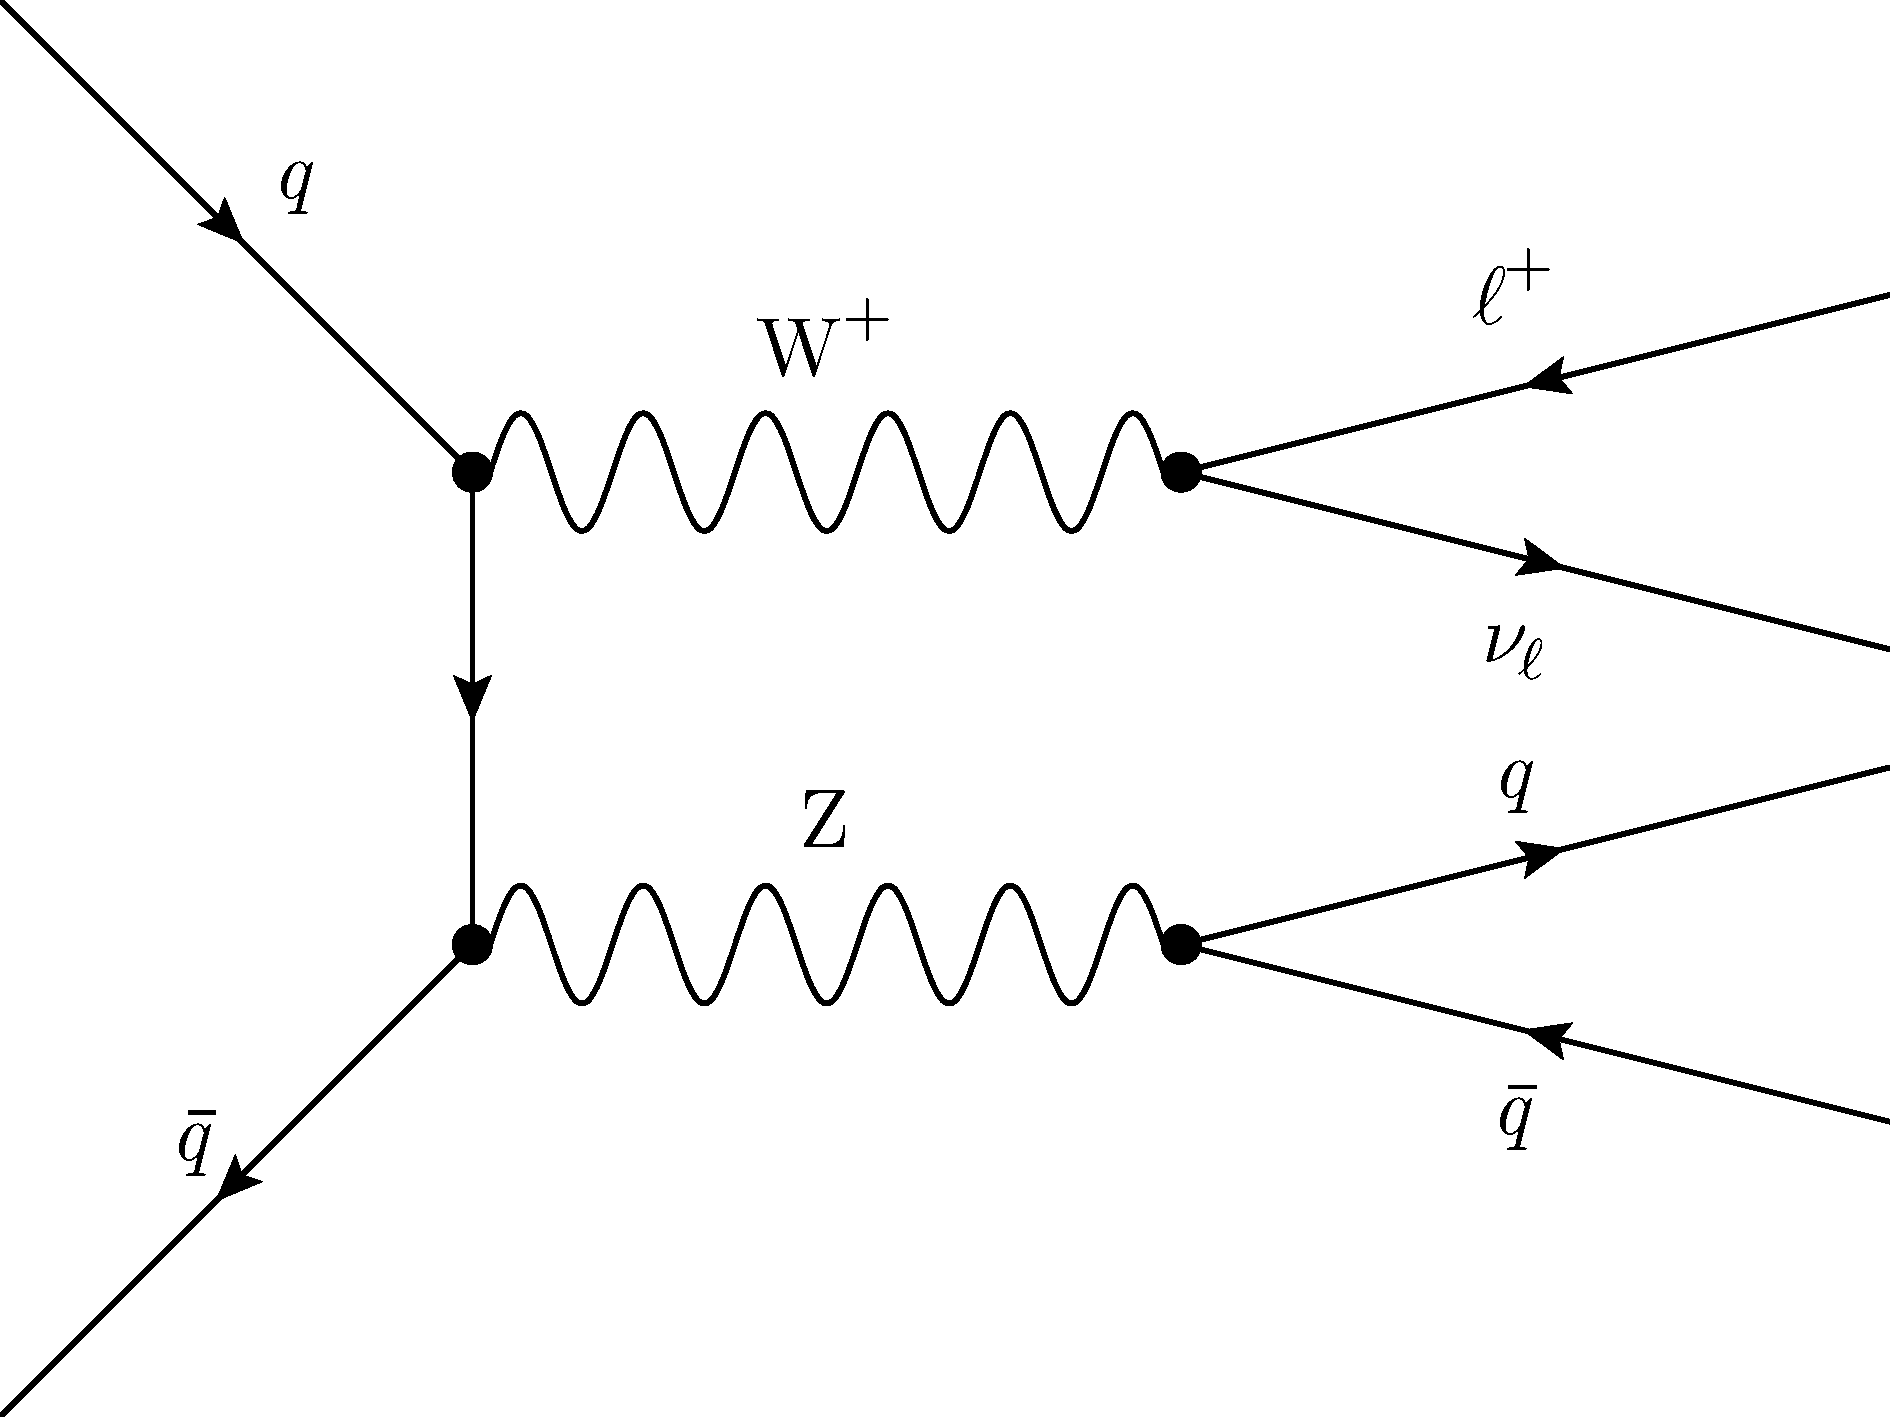
\includegraphics[width=0.25\textwidth]{\figpath/FeynmanDiagrams/WZ.pdf} & & \\
		\end{tabular}
	\end{table}
	\vspace*{-0.2cm}
	\begin{itemize}
		\item \textit{\textbf{Reducible}} backgrounds are those with fake (extra) leptons or b-jets
	\end{itemize}
	\vspace*{-0.2cm}
	\begin{table}[tb]
		\centering
		\begin{tabular}{>{\centering}m{0.15\textwidth} >{\centering}m{0.27\textwidth} | >{\centering}m{0.15\textwidth} >{\centering\arraybackslash}m{0.27\textwidth}}
			  \ttbar & 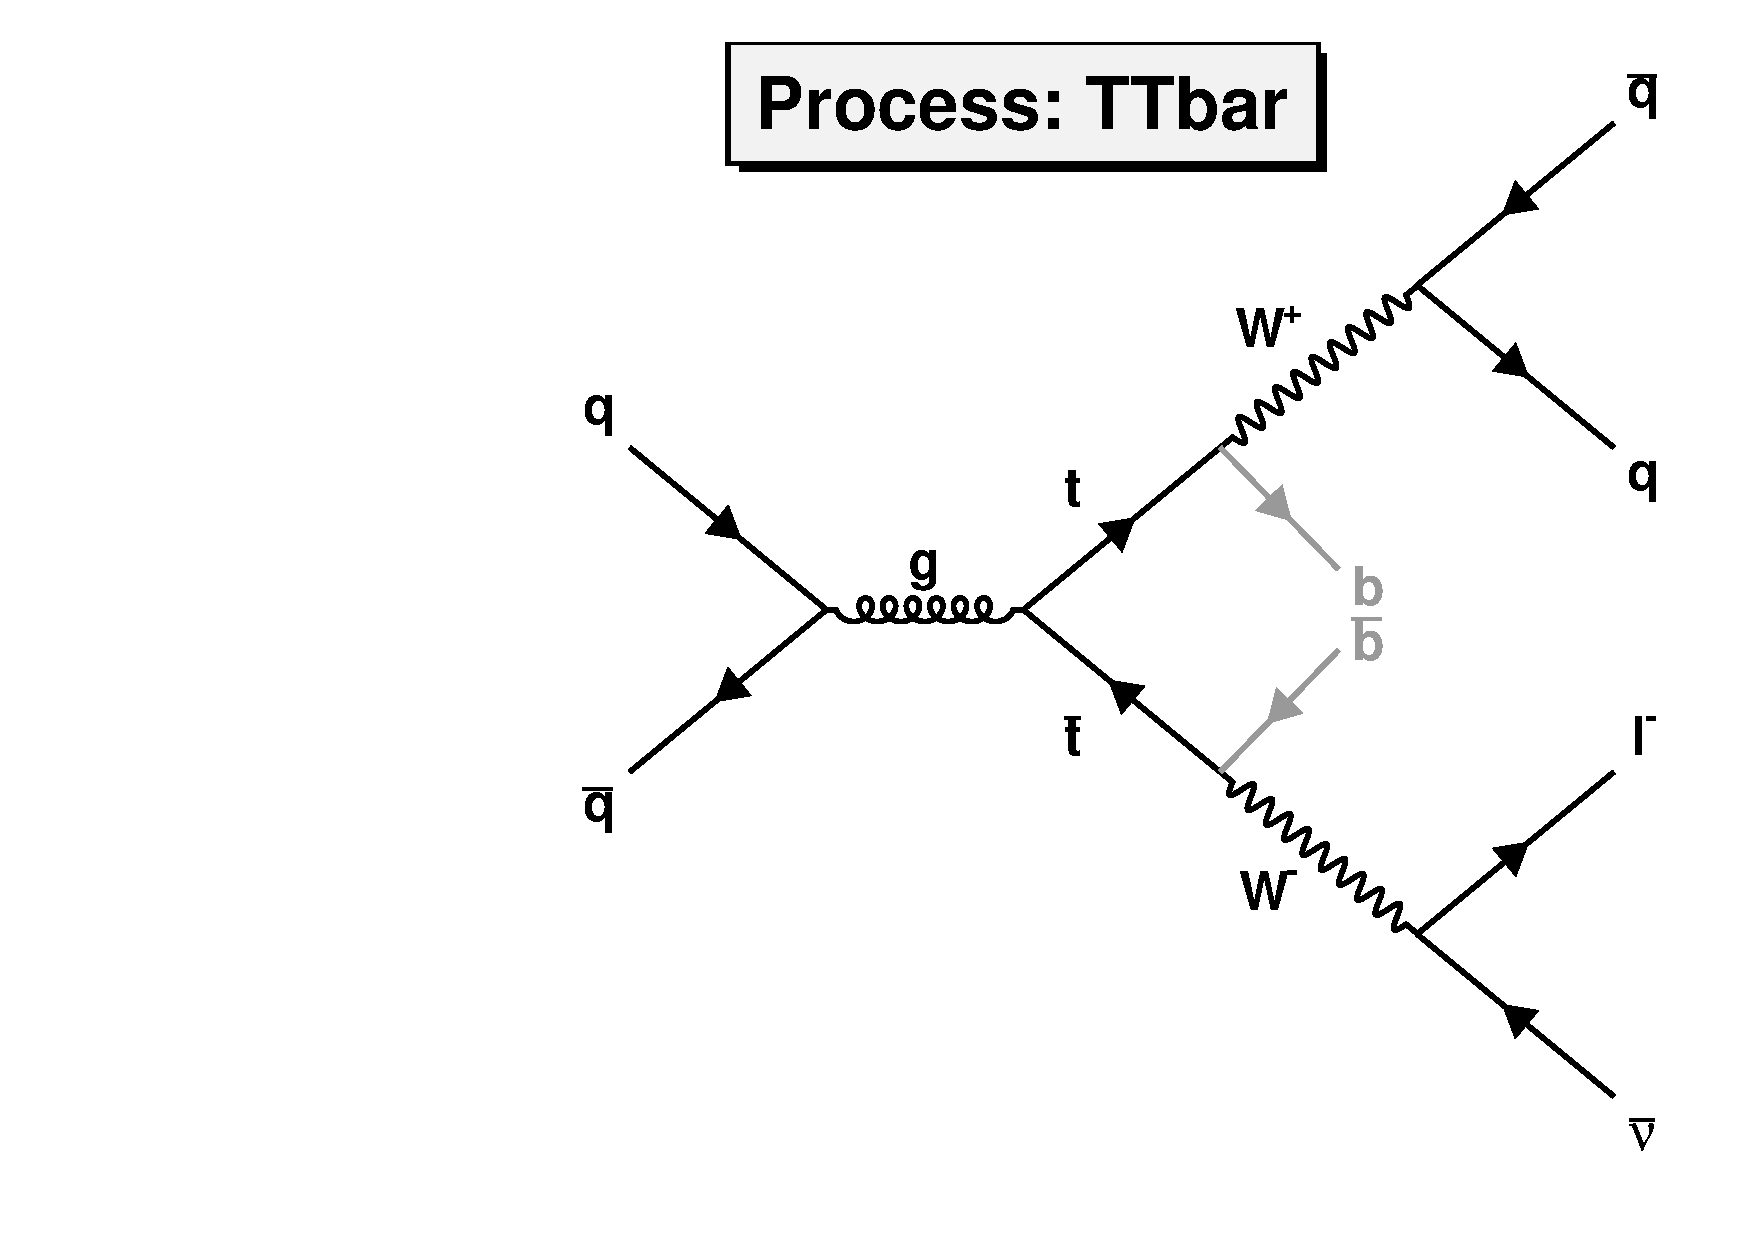
\includegraphics[width=0.25\textwidth]{\figpath/FeynmanDiagrams/TTbar.pdf} & & \\
		\end{tabular}
	\end{table}
\end{frame}

\begin{frame}
	\frametitle{SM Backgrounds}
	\vspace*{-0.24cm}
	\begin{itemize}
		\item \textit{\textbf{Reducible}} backgrounds continued \ldots
	\end{itemize}
	\begin{table}[tb]
		\centering
		\begin{tabular}{>{\centering}m{0.15\textwidth} >{\centering}m{0.27\textwidth} | >{\centering}m{0.15\textwidth} >{\centering\arraybackslash}m{0.27\textwidth}}
			\Zjets & 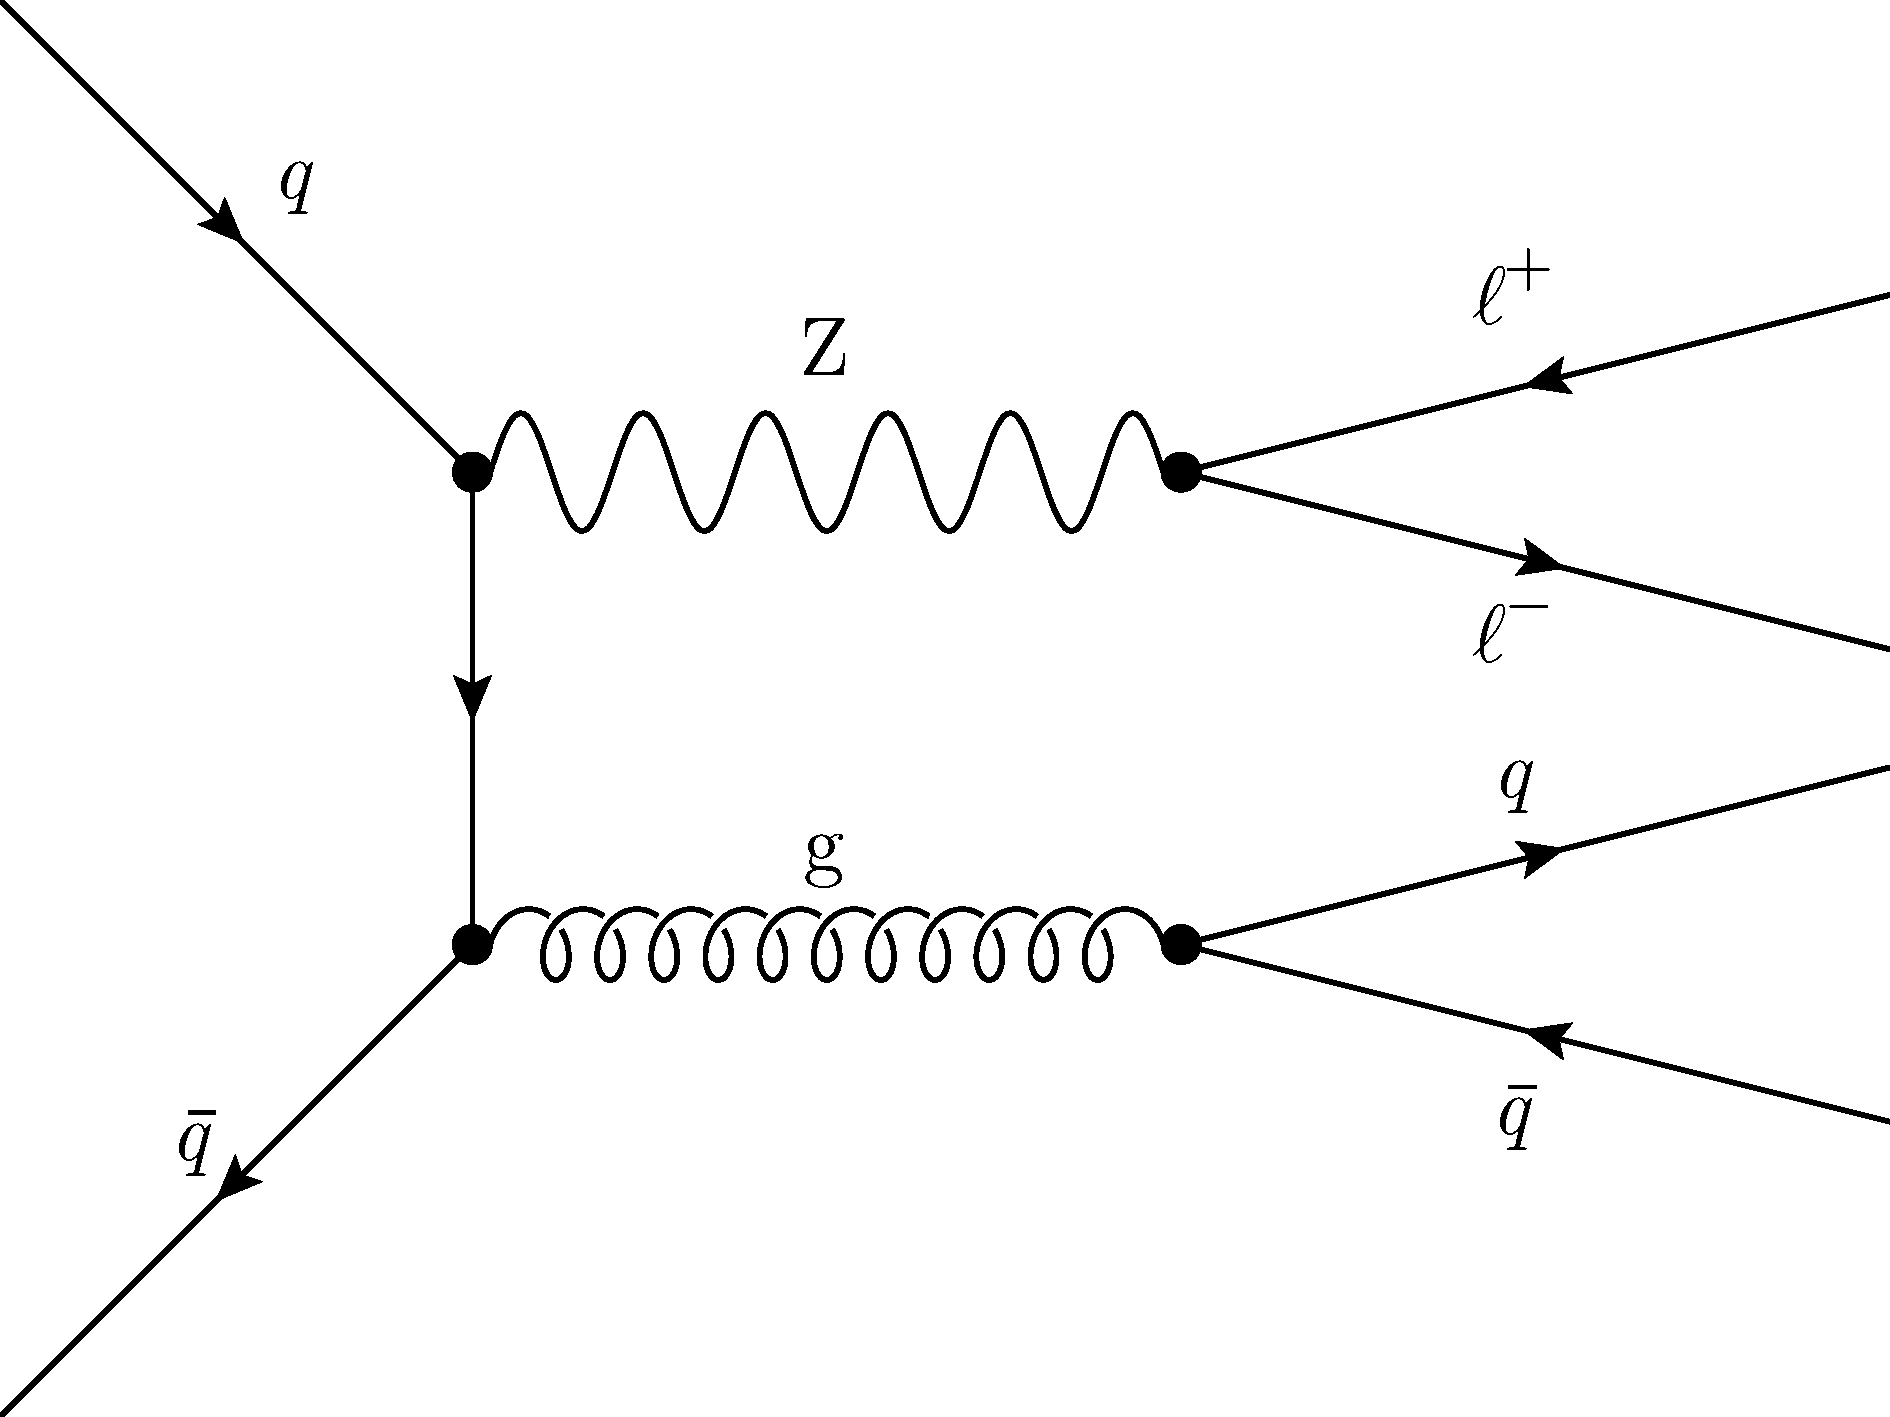
\includegraphics[width=0.25\textwidth]{\figpath/FeynmanDiagrams/ZJets.pdf} & \ZZ & 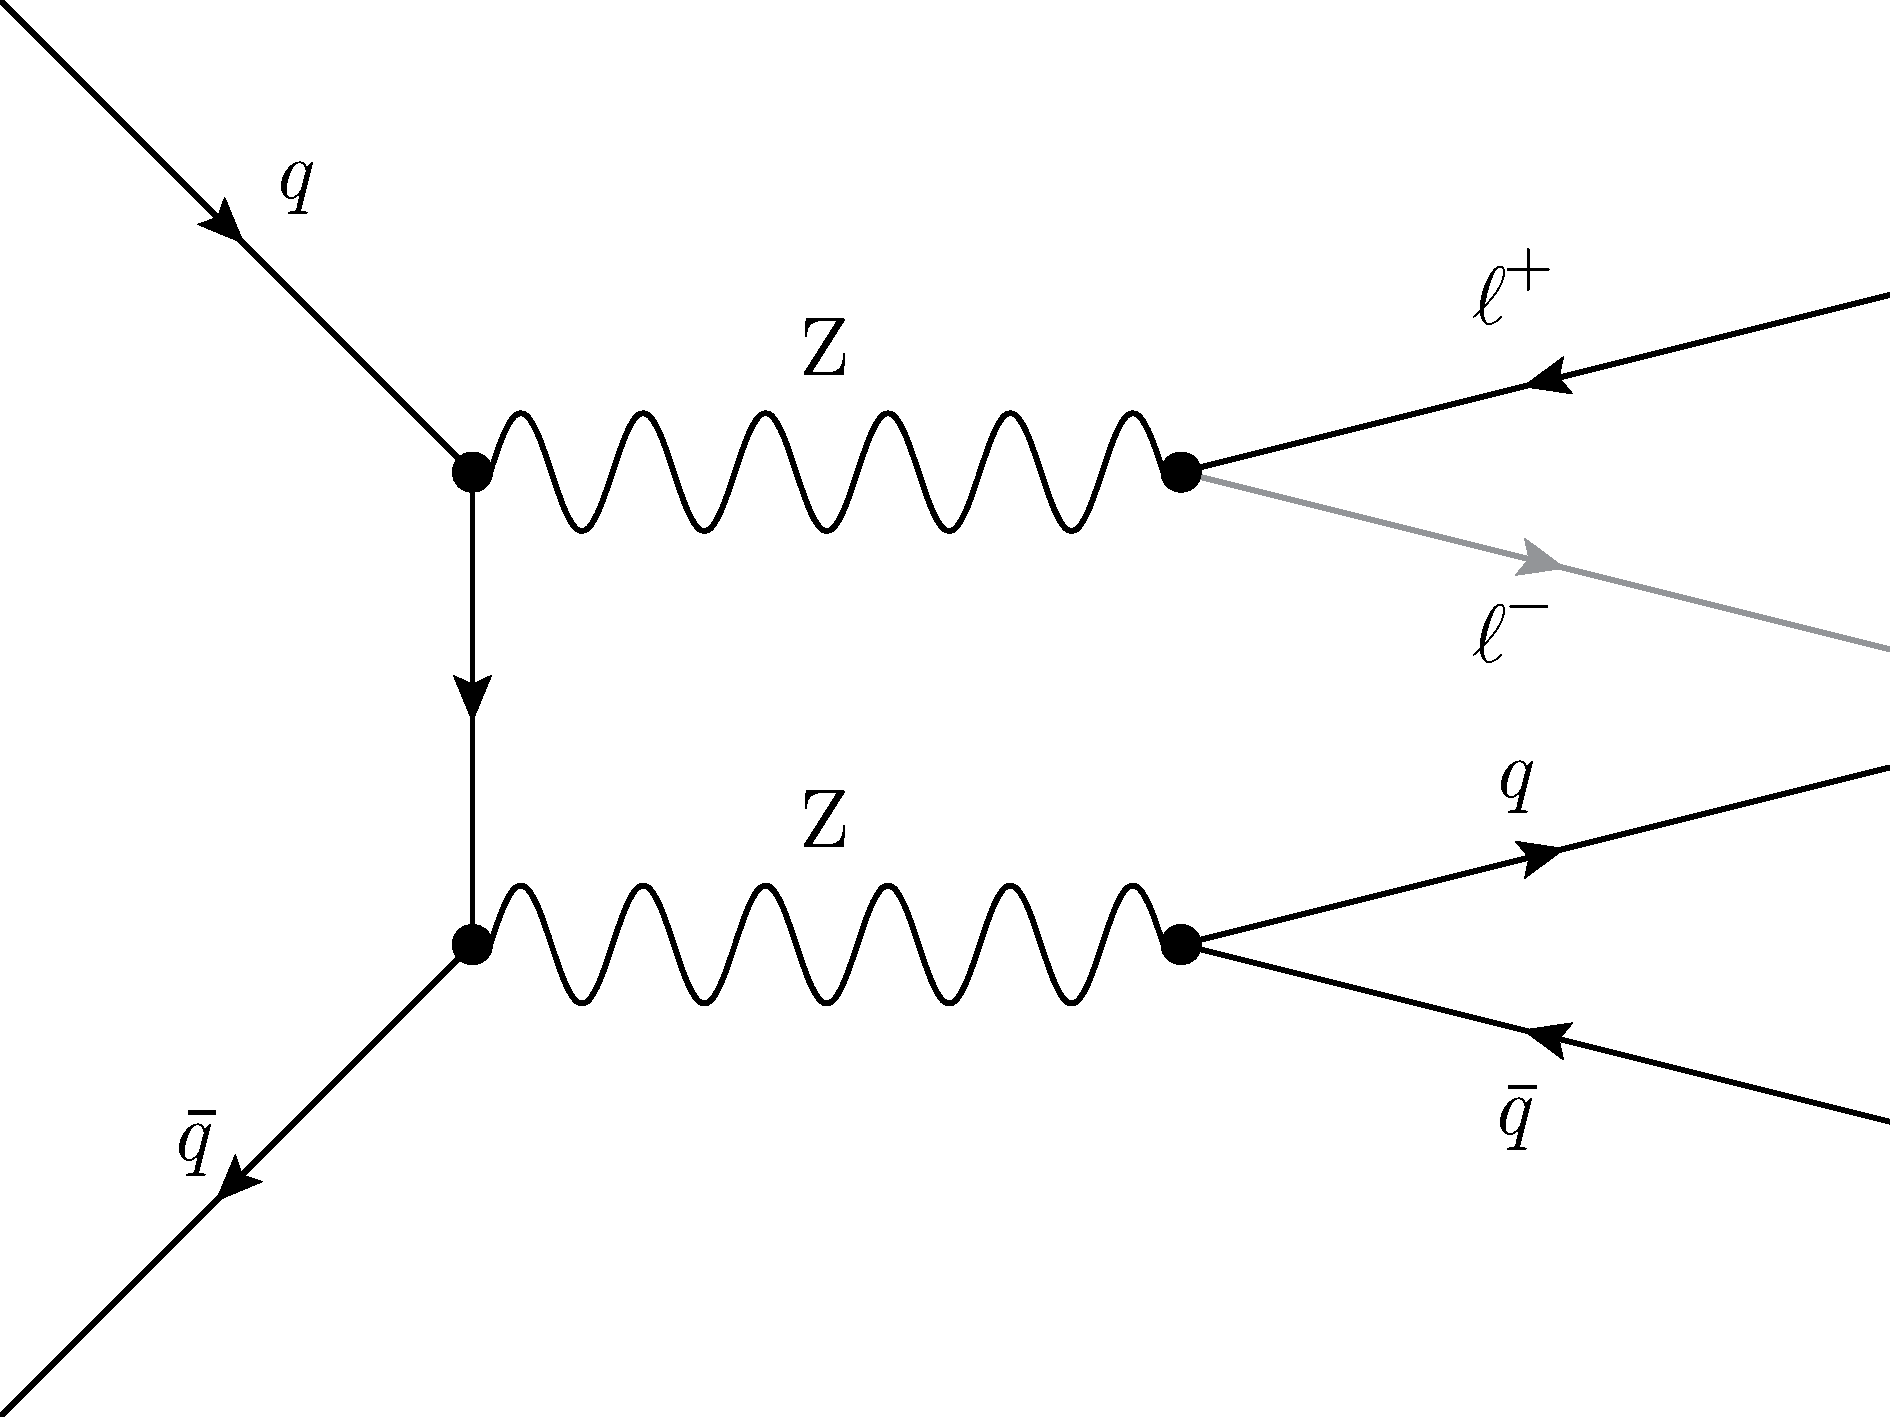
\includegraphics[width=0.25\textwidth]{\figpath/FeynmanDiagrams/ZZ.pdf} \\
			Single-\cPqt\\(\cPqs-channel) & 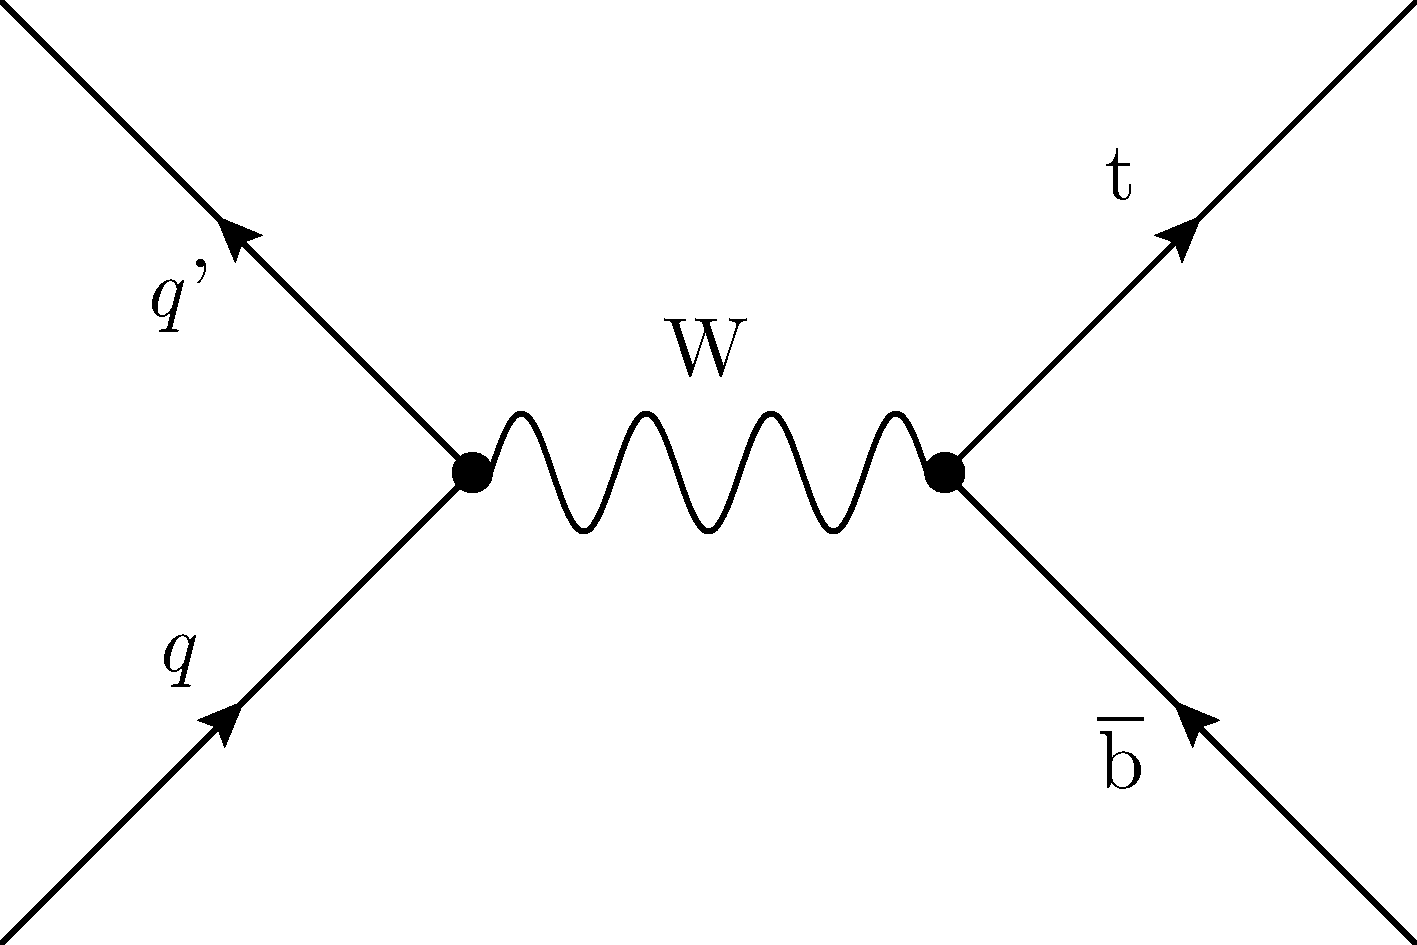
\includegraphics[width=0.25\textwidth]{\figpath/FeynmanDiagrams/STopS.pdf} & Single-\cPqt\\(\cPqt-channel) & 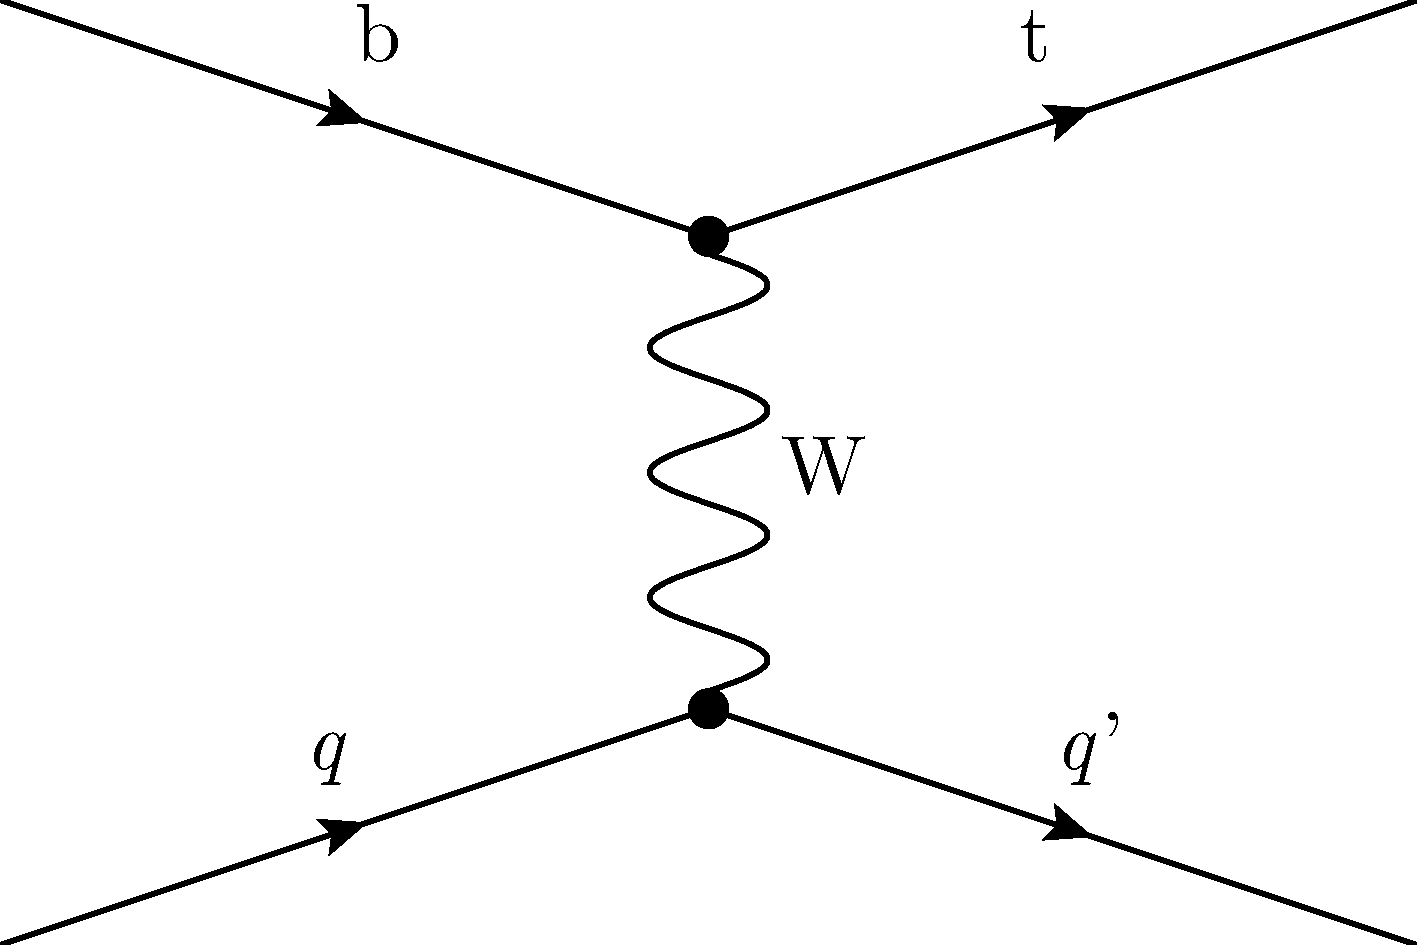
\includegraphics[width=0.25\textwidth]{\figpath/FeynmanDiagrams/STopT.pdf} \\
			Single-\cPqt\\(\cPqt\PW-channel) & 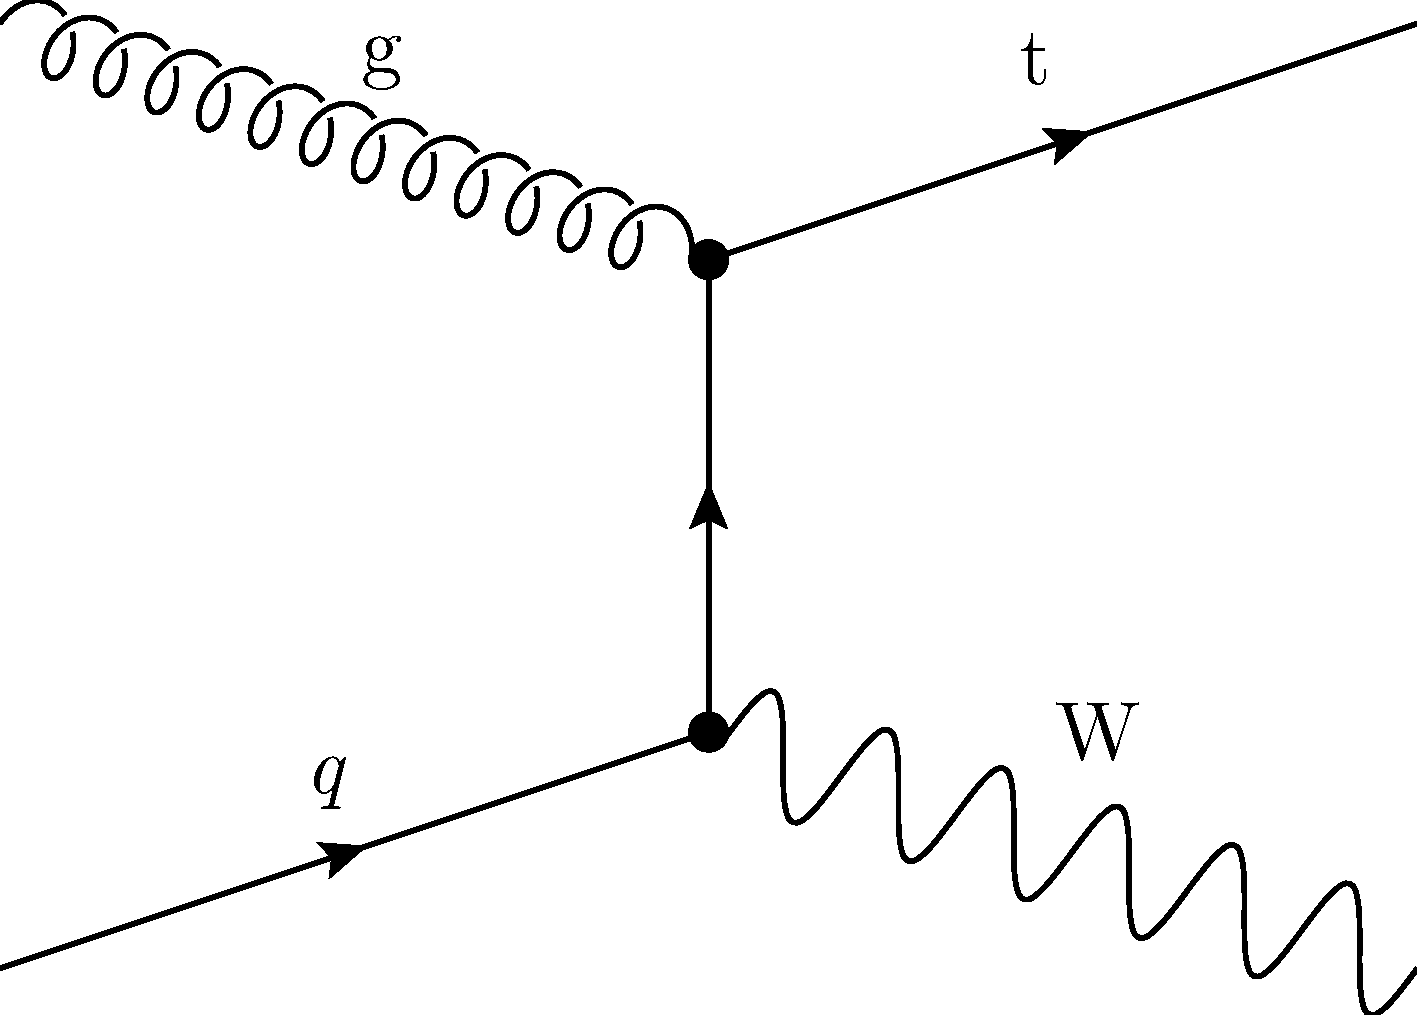
\includegraphics[width=0.25\textwidth]{\figpath/FeynmanDiagrams/STopTW.pdf} & QCD & 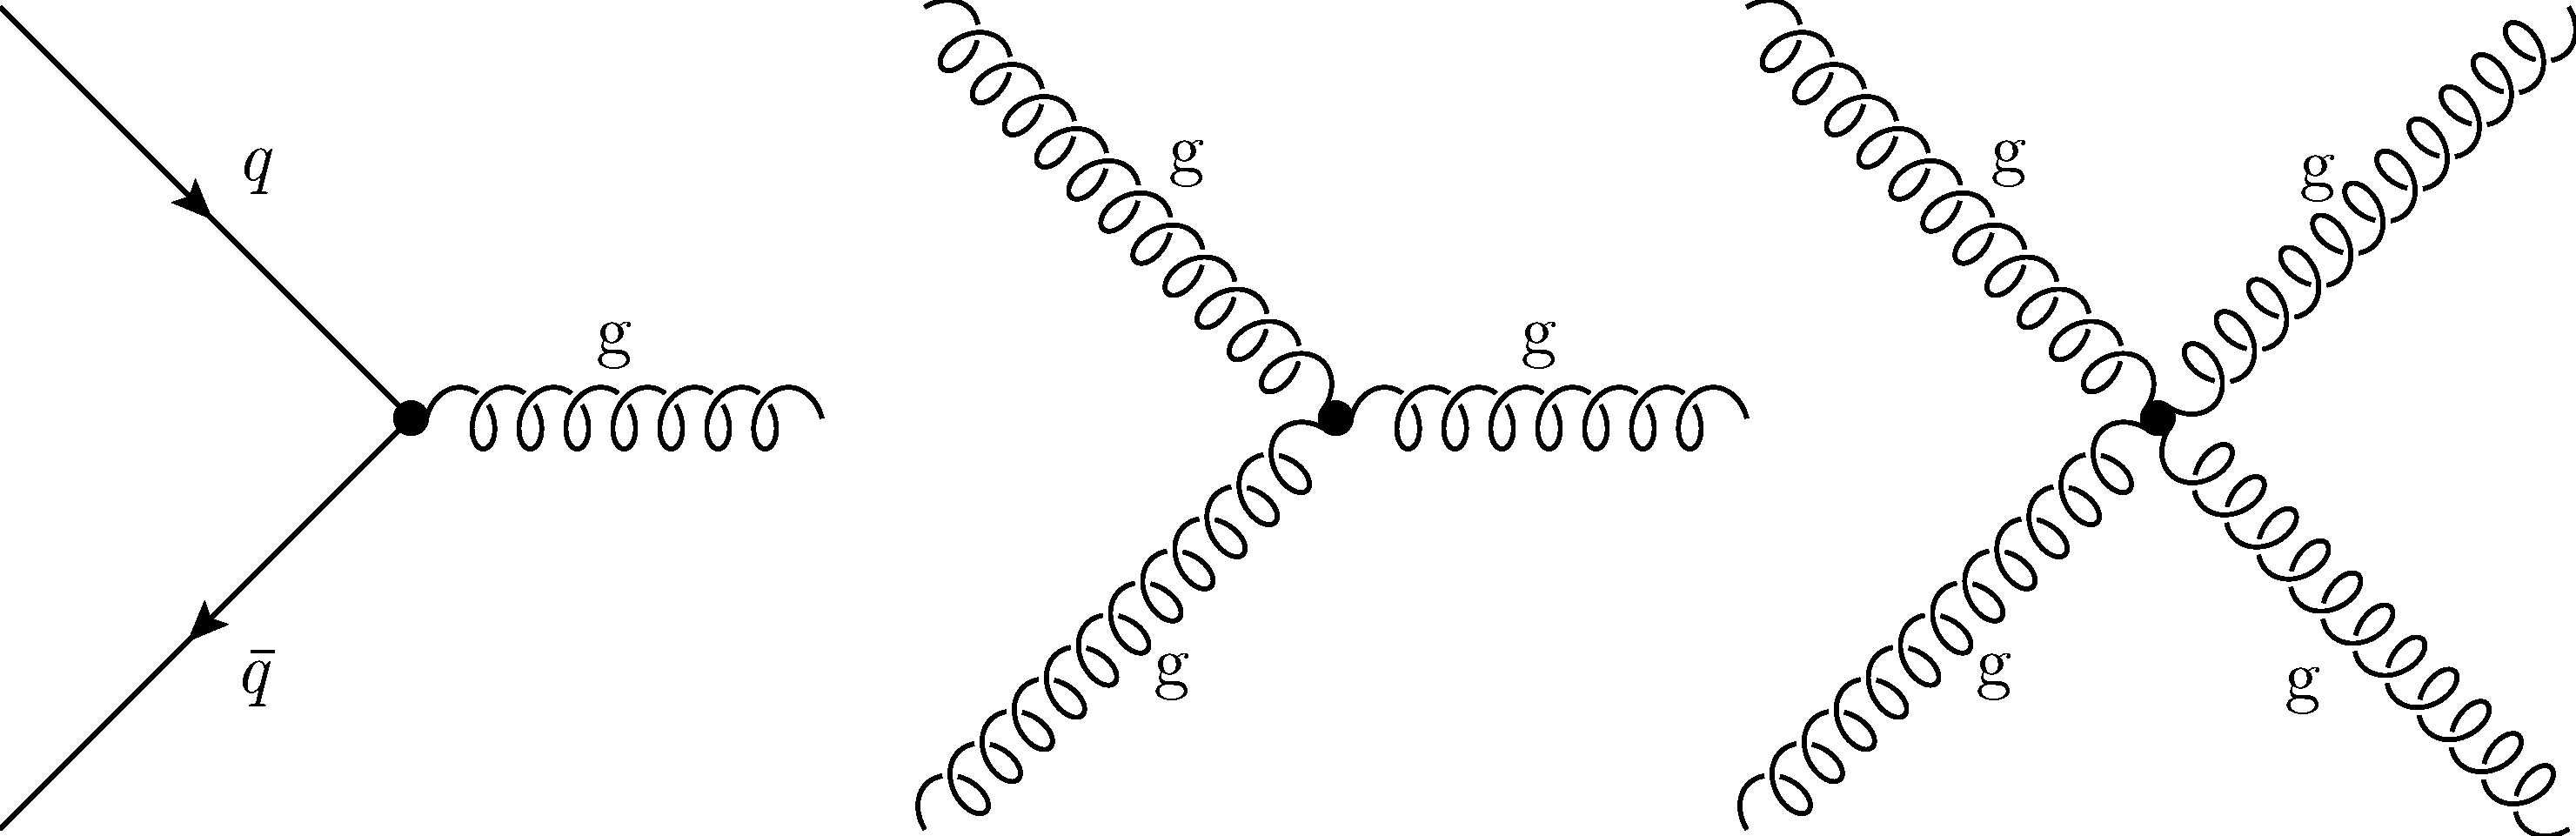
\includegraphics[width=0.25\textwidth]{\figpath/FeynmanDiagrams/QCD.pdf}\\
		\end{tabular}
	\end{table}
\end{frame}